\documentclass[]{article}
\usepackage{lmodern}
\usepackage{amssymb,amsmath}
\usepackage{ifxetex,ifluatex}
\usepackage{fixltx2e} % provides \textsubscript
\ifnum 0\ifxetex 1\fi\ifluatex 1\fi=0 % if pdftex
  \usepackage[T1]{fontenc}
  \usepackage[utf8]{inputenc}
\else % if luatex or xelatex
  \ifxetex
    \usepackage{mathspec}
  \else
    \usepackage{fontspec}
  \fi
  \defaultfontfeatures{Ligatures=TeX,Scale=MatchLowercase}
\fi
% use upquote if available, for straight quotes in verbatim environments
\IfFileExists{upquote.sty}{\usepackage{upquote}}{}
% use microtype if available
\IfFileExists{microtype.sty}{%
\usepackage{microtype}
\UseMicrotypeSet[protrusion]{basicmath} % disable protrusion for tt fonts
}{}
\usepackage{hyperref}
\hypersetup{unicode=true,
            pdftitle={MAS341 Lecture Notes 2016},
            pdfborder={0 0 0},
            breaklinks=true}
\urlstyle{same}  % don't use monospace font for urls
\usepackage{graphicx,grffile}
\makeatletter
\def\maxwidth{\ifdim\Gin@nat@width>\linewidth\linewidth\else\Gin@nat@width\fi}
\def\maxheight{\ifdim\Gin@nat@height>\textheight\textheight\else\Gin@nat@height\fi}
\makeatother
% Scale images if necessary, so that they will not overflow the page
% margins by default, and it is still possible to overwrite the defaults
% using explicit options in \includegraphics[width, height, ...]{}
\setkeys{Gin}{width=\maxwidth,height=\maxheight,keepaspectratio}
\IfFileExists{parskip.sty}{%
\usepackage{parskip}
}{% else
\setlength{\parindent}{0pt}
\setlength{\parskip}{6pt plus 2pt minus 1pt}
}
\setlength{\emergencystretch}{3em}  % prevent overfull lines
\providecommand{\tightlist}{%
  \setlength{\itemsep}{0pt}\setlength{\parskip}{0pt}}
\setcounter{secnumdepth}{0}
\setcounter{tocdepth}{1}
% Redefines (sub)paragraphs to behave more like sections
\ifx\paragraph\undefined\else
\let\oldparagraph\paragraph
\renewcommand{\paragraph}[1]{\oldparagraph{#1}\mbox{}}
\fi
\ifx\subparagraph\undefined\else
\let\oldsubparagraph\subparagraph
\renewcommand{\subparagraph}[1]{\oldsubparagraph{#1}\mbox{}}
\fi

\title{MAS341 Graph Theory \\ Lecture Notes}
\date{}

\begin{document}
\maketitle
\tableofcontents


\section{Lecture 1: Introduction and Euler's Handshaking Lemma}
\subsubsection{Graphs}\label{graphs}

Graphs usually (but not always) are thought of showing how things are
set of things are connected together.

\subsection{Definition of a graph}\label{definition-of-a-graph}

A \emph{graph} \(\Gamma\) consists of:

\begin{itemize}
\tightlist
\item
  a set \(V(\Gamma)\) of vertices
\item
  a set \(E(\Gamma)\) of edges
\end{itemize}

Each edge either connects two vertices of \(V(\Gamma)\) together, or
connects a vertex to itself.

\subsection{Examples}\label{examples}

See the slides for many picture examples, but here are some common
examples:

\begin{itemize}
\tightlist
\item
  cities as vertices and roads connecting them as edges
\item
  people as vertices and an edge between two people if they know each
  other
\item
  atoms in a molecule as vertices, with an edge between them if they are
  connected by a covalent bond
\item
  countries on a map as vertices, and shared borders as edges
\end{itemize}

\subsection{A few more definitions}\label{a-few-more-definitions}

There are two features of graphs that are sometimes convenient to not
allow.

A \emph{loop} is an edge that connects a vertex to itself, and a
\emph{multiple edge} is when there is more than one edge connecting the
same two vertices. A graph without these features is called
\emph{simple}.

We say two vertices are \emph{adjacent} if there is an edge between
them.

The \emph{degree} or \emph{valency} of a vertex in a simple graph is the
number of vertices it is adjacent to.

\subsubsection{A first question}\label{a-first-question}

Suppose you are at a party with six other people, so that there are
seven people total at the party. Is it possible that everybody knows
exactly three other people at the party?

To translate this into graph theory, we make the people vertices, and
put an edge between two people if they know each other. We are then
asking if a graph exists with seven vertices, where each vertex has
degree three.

It turns out that this is not possible; one way to prove this would be
doing a case by case analysis of trying to make such a graph, but such
proofs are usually long, messy, and not particularly enlightening.

Instead, we argued as follows: suppose that everyone at the party shook
hands with the people they knew, but not with the people they don't
know. How many handshakes would occur?

It is immediate from the definition that the number of handshakes would
be the number of edges in the graph. But we could also count the number
of handshakes in another way: each person is going to shake hands three
times, so people will be involved in handshakes 3*7=21 times. But since
each handshake involves two people, this should be twice the number of
handshakes. From this reasoning, we see there should be 21/2=10.5 edges
in the graph, which is absurd, and so we see that such a party is not
possible.

The argument given above easily generalizes to give

\subsection{Euler's handshaking lemma:}\label{eulers-handshaking-lemma}

The sum of the degrees of the vertices of a graph is twice the number of
edges of the graph:

\(\sum_{v\in V(\Gamma)}d(v)=2|E(\Gamma)|\)

\subsection{Proof:}\label{proof}

Each edge has two ends; each end contributes 1 to the degree of one
vertex, and hence to the sum of all the degrees. \(\square\)

\subsubsection{Graph theory in Chemistry}\label{graph-theory-in-chemistry}

In organic chemistry, atoms are joined together by covalent bonds; we
represent this in a graph with the atoms as vertices and the edges
representing the bonds. The location of the element on the periodic
table determines the valency of the vertices corresponding to that
element:

\begin{itemize}
\tightlist
\item
  Hydrogen (H) and Fluorine (F) have degree 1
\item
  Oxygen (O) and Sulfur (S) have degree 2
\item
  Nitrogen (N) and Phosphorous (P) have degree 3
\item
  Carbon (C) has degree 4
\end{itemize}

Usually, most of the atoms involved are carbon and hydrogen. Carbon
atoms are not labelled with a C, but just left blank, while hydrogen
atoms are left off completely. One can then complete the full structure
of the molecule using the valency of each vertex.

Graphs coming from organic chemistry do not have to be simple --
sometimes there are double bonds, where a pair of carbon atoms have two
edges between them.

\subsection{Definition: degree sequence}\label{definition-degree-sequence}

The \emph{degree sequence} of a graph is just the list (with
multiplicity) of the degrees of all the vertices.

\subsubsection{\texorpdfstring{So, knowing the chemical composition of a
molecule determines the degree sequence of its corresponding graph.
However, it is possible that the same set of atoms may be put together
into a molecule in more than one different ways. In terms of graphs,
this corresponds to ``different'' graphs that have the same degree
sequence.}{So, knowing the chemical composition of a molecule determines the degree sequence of its corresponding graph. However, it is possible that the same set of atoms may be put together into a molecule in more than one different ways. In terms of graphs, this corresponds to different graphs that have the same degree sequence.}}\label{so-knowing-the-chemical-composition-of-a-molecule-determines-the-degree-sequence-of-its-corresponding-graph.-however-it-is-possible-that-the-same-set-of-atoms-may-be-put-together-into-a-molecule-in-more-than-one-different-ways.-in-terms-of-graphs-this-corresponds-to-different-graphs-that-have-the-same-degree-sequence.}

\section{Lecture 2: Instant Insanity, Isomorphisms }

\subsubsection{Instant Insanity}\label{instant-insanity}

A concrete, nontrivial application of graph theory is as a tool to solve
the puzzle ``instant insanity'', known sometimes as the four cubes
problem.

\subsection{Basic setup}\label{basic-setup}

In this puzzle, one is given four cubes. Each face of each cube is
painted one of four different colours: blue, green, red or yellow. The
goal is to line the four cubes up in a row, so that along the four long
edges (front, top, back, bottom) each of the four colours appears eactly
once.

Depending on how the cubes are coloured, this may be not be possible, or
there may be many such possibilities. In the original instant insanity,
there is exactly one solution. I have made a video that explains how to
use graph theory to show the solution to the original onstant insanity.

There are many variations on Instant Insanity, discussion of which can
be found, for
\href{http://www.cs.brandeis.edu/~storer/JimPuzzles/ZPAGES/zzzInstantInsanity.html}{here}
and \href{http://www.jaapsch.net/puzzles/insanity.htm}{here}. There's
also \href{https://www.youtube.com/watch?v=CQ2gHSKZBEw}{a commercial}
for the game.

\subsubsection{An impossible example}\label{an-impossible-example}

In lecture, I walked through proving that the following example has no
solutions. The work was done on the board and not in the slides, but I
will present the work here.

The four cubes in question are:

\subsection{Enter graph theory}\label{enter-graph-theory}

We will now construct a graph that encodes the important part of the
structure of the cubes.

The vertices of the graph will be the four colors, B, G, R and Y. We
will put an edge between two colors each time they appear as opposite
faces on a cube, and we will label that edge with a number 1-4 denoting
which cube the two opposite faces appear. So from the first cube, there
will be a loop at B, and edge between G and R, and an edge between Y and
R.

The graph corresponding to the four cubes above is the following:

\subsection{Proving our cubes were
impossible}\label{proving-our-cubes-were-impossible}

How does this graph help us study the solutions of the Instanity
Insanity puzzle? Suppose we had an arrangement of the cubes that was a
solution. Then, from each cube, pick the edge representing the colors
facing front and back on that cube. These four edges are a subgraph of
our original graph, with one edge of each label, since we picked one
edge from each cube. Furthermore, since we assumed the arrangement of
cubes was a solution of instant insanity, each color appears once on the
front face and once on the back. In terms of our subgraph, this
translates into asking that each vertex has degree two.

We got another subgraph satisfying these two properties by looking at
the faces on the top and bottom for each cube and taking the
corresponding edges. Furthermore, these two subgraphs do not have any
edges in common.

Thus, given a solution to the instant insanity problem, we found a pair
of subgraphs \(S_1, S_2\) satisfying:

\begin{enumerate}
\def\labelenumi{\arabic{enumi}.}
\tightlist
\item
  Each subgraph \(S_i\) has one edge with each label 1,2,3,4
\item
  Every vertex of \(S_i\) has degree 2
\item
  No edge of the original graph is used in both \(S_1\) and \(S_2\)
\end{enumerate}

As an exercise, one can check that given a pair of subgraphs satisfying
1-3, one can produce a solution to the instant insanity puzzle.

Thus, to show the set of cubes we are currently examining does not have
a solution, we need to show that the graph does not have two subgraphs
satisfying properties 1-3.

To do, this, we catalog all graphs satisfying properties 1-2. If every
vertex has degree 2, either

\begin{enumerate}
\def\labelenumi{\arabic{enumi}.}
\tightlist
\item
  Every vertex has a loop
\item
  There is one vertex with a loop, and the rest are in a triangle
\item
  There are two vertices with loops and a double edge between the other
  two vertices
\item
  There are two pairs of double edges
\item
  All the vertices live in one four cycle
\end{enumerate}

A subgraphs of type 1 is not possible, because G and R do not have
loops.

For subgraphs of type 2, the only triangle is G-R-Y, and B does have
loops. The edge between Y-G must be labeled 3, which means the loop at B
must be labeled 1. This means the edge between G and R must be labeled 4
and the edge between Y and R must be 2, giving the following subgraph:

For type 3, the only option is to have loops at B and Y and a double
edge between G and R. We see the loop at Y must be labeled 2, one of the
edges between G and R must be 4, and the loop at B and the other edge
between G and R can switch between 1 and 3, giving two possibilities:

and

For subgraphs of type 4, the only option would be to have a double edge
between B and G and another between Y and R; however, none of these
edges are labeled 3 and this option is not possible.

Finally, subgraphs of type 5 cannot happen because B is only adjacent to
G and to itself; to be in a four cycle it would have two be adjacent to
two vertices that aren't itself.

This gives three different possibilities for the subgraphs \(S_i\) that
satisfy properties 1 and 2. However, all three possibilities contain the
the edge labeled 4 between G and R; hence we cannot choice two of them
with disjoint edges, and the instant insanity puzzle with these cubes
does not have a solution.

\subsubsection{\texorpdfstring{Isomorphisms: When are two graphs ``the
same''?}{Isomorphisms: When are two graphs the same?}}\label{isomorphisms-when-are-two-graphs-the-same}

It is possible to draw the same graph in the plane in many different
ways -- e.g., the pentagon and the five sided star are two different
ways of drawing \(C_5\).

If two graphs are ``the same'' in this way, we say they are
\emph{isomorphic}.

\subsection{Definition}\label{definition}

An \emph{isomorphism} \(\varphi:G\to H\) of simple graphs is a bijection
\(\varphi:V(G)\to V(H)\) that preserves the number of edges between
vertices. That is, if \(v,w\in V(G)\), then the number of edges between
\(v\) and \(w\) in \(G\) is equal to the number of edges between
\(\varphi(v)\) and \(\varphi(w)\) in \(H\).

\subsection{Example}\label{example}

This animated gif shows several graphs isomorphic to the Petersen graph,
and demonstrates that they are isomorphic:

\subsubsection{Graph isomorphism problem}\label{graph-isomorphism-problem}

The \emph{graph isomorphism problem} is to decide whether or not two
given graphs \(G, H\) are isomorphic.

\subsection{General discussion for mathematical cultural
literacy}\label{general-discussion-for-mathematical-cultural-literacy}

The isomorphism problem is of fundamental importance to theoretical
computer science. Apart from its practical applications, the exact
difficulty of the problem is unknown. Clearly, if the graphs are
isomorphic, this fact can be easily demonstrated and checked, which
means the Graph Isomorphism is in NP.

Most problems in NP are known either to be easy (solvable in polynomial
time, P), or at least as difficult as any other problem in NP (NP
complete). This is not true of the Graph Isomorphism problem. In
November of last year, Laszlo Babai announced a quasipolynomial-time
algorithm for the graph isomorphism problem -- you can read about this
work in
\href{https://www.quantamagazine.org/20151214-graph-isomorphism-algorithm/}{this
great popular science article}.

\subsection{What you have to be able to
do}\label{what-you-have-to-be-able-to-do}

Although solving the graph isomorphism problem for general graphs is
quite difficult, doing it for small graphs by hand is not too bad and is
something you must be able to do for the exam.

If the two graphs are actually isomorphic, you have to actually write
down an explicit isomorphism \(\varphi:G\to H\) should be given.

If they are not isomorphic, you have to prove that they are not
isomorphic. Usually this is done by giving an \emph{obstruction} --
something that is different between the two graphs. One easy example is
that isomorphic graphs have to have the same number of edges and
vertices.

Another, only slightly more advanced invariant is the degree sequence of
a graph that we saw last lecture in our discussion of chemistry.

If \(\varphi:G \to H\) is an isomorphism of graphs, than we must have
\(d(\varphi(v))=d(v)\) for all vertices \(v\), and so the degree
sequence must be preserved. However, just because two graphs have the
same degree sequences does not mean they are isomorphic.

\section{Lecture 3: Connectedness.  Walks, trails and paths}

If the edges in a graph \(\Gamma\) represent connections, it is obvious
to ask whether \(\Gamma\) as a whole is ``connected''. There are two
seemingly different ways of making this precise; today we introduce
these and show that they are the same.

It may be easiest to define what it means for a graph \(\Gamma\) to be
\emph{disconnected}.

\subsection{Definition: Disjoint union}\label{definition-disjoint-union}

Given two graphs \(\Gamma_1\) and \(\Gamma_2\), the \emph{disjoint
union} \(\Gamma_1\sqcup \Gamma_2\) is obtained by taking the disjoint
union of both the vertices and edges of \(\Gamma_1\) and \(\Gamma_2\).
So \(\Gamma_1\sqcup\Gamma_2\) consists of a copy of \(\Gamma_1\) and a
copy of \(\Gamma_2\), with no edges in between the two graphs.

\subsection{Definition: Disconnected}\label{definition-disconnected}

A graph \(\Gamma\) is \emph{disconnected} if we can write
\(\Gamma=\Gamma_1\sqcup \Gamma_2\) for two proper (i.e., not all of
\(\Gamma\)) subgraphs \(\Gamma_1\) and \(\Gamma_2\).

It then makes sense to say that \(\Gamma\) is \emph{connected} if it is
not disconnected. However, the more intuitive notion of being connected
is that ``you can get from any vertex to any other'', which we now make
precise.

\subsubsection{Walks, Trails, Paths}\label{walks-trails-paths}

\subsection{Definition}\label{definition-1}

A \emph{walk} in a graph \(\Gamma\) is a sequence

\[v_0, e_1, v_1,e_2, v_2,\dots, v_{n-1}, e_n, v_n\]

where - the \(v_i\) are vertices - the \(e_j\) are edges - edge \(e_j\)
goes between vertices \(v_{j-1}\) and \(v_j\)

Note that, when the graph \(\Gamma\) does not have multiple edges, it is
enough to record just the \(v_i\), but if \(\Gamma\) has multiple edges
that just knowing the vertices does not determine the walk.

We say that the walk is between vertices \(a\) and \(b\) if \(a=v_0\) to
vertex \(b=v_n\). Thus, it is natural to say that a graph \(\Gamma\) is
connected if there is a walk between any two vertices \(a,b\in\Gamma\).
We now show that this agrees with our previous definition of connected.

\subsection{Lemma}\label{lemma}

The following are equivalent:

\begin{enumerate}
\def\labelenumi{\arabic{enumi}.}
\tightlist
\item
  \(\Gamma\) is connected.
\item
  There is a walk between any two vertices \(v, w\in V(\Gamma)\)
\end{enumerate}

\subsection{Proof}\label{proof-1}

1 implies 2: Supppose that \(\Gamma\) is connected, and let
\(v, w\in V(\Gamma)\); we want to show that there is a walk from \(v\)
to \(w\).

Define \(S\subset V(\Gamma)\) to be the set of all vertices
\(u\in V(\Gamma)\) so that there is a walk from \(v\) to \(u\); we want
to show that \(w\in S\).

First, observe that there are no edges from \(S\) to
\(V(\Gamma)\setminus S\). Suppose that \(e\) was an edge between
\(a\in S\) and \(b\in\Gamma\setminus S\). Since \(a\in S\), by the
definition of \(S\) there is a walk \(v=v_0v_1v_2\cdots v_m=a\) from
\(v\) to \(a\). We can add the edge \(e\) to the end of the walk, to get
a walk from \(v\) to \(b\), and hence by definition \(b\in S\).

Now suppose that \(w\notin S\). Then \(S\) and \(V(\Gamma)\setminus S\)
are both nonempty, and by the above there are no edges between them, and
so \(\Gamma\) is not connected, a contradiction.

To prove 2 implies 1, we prove the contrapositive. If \(\Gamma\) is not
connected, then there are two vertices \(v,w\in V(\Gamma)\) so that
there is no walk from \(v\) to \(w\).

Suppose that \(\Gamma=\Gamma_1\sqcup\Gamma_2\), and pick
\(v\in V(\Gamma_1), w\in V(\Gamma_2)\). Any walk from \(v\) to \(w\)
starts in \(V(\Gamma_1)\) and ends in \(V(\Gamma_2)\), and so at some
point there must be an edge from a vertex in \(\Gamma_1\) to a vertex in
\(\Gamma_2\), but there are no such edges \(\square\)

\subsubsection{Types of Walks}\label{types-of-walks}

Many questions in graph theory ask whether or not a walk of a certain
type exists on a graph: we introduce some notation that will be needed
for these questions.

We say a walk is \emph{closed} if it starts and ends on the same vertex;
i.e., \(v_0=v_n\). The \emph{length} of a walk is \(n\), the number of
edges in it. The \emph{distance} between two vertices \(v\) and \(w\) is
the length of the shortest walk from \(v\) to \(w\), if one exists, and
\(\infty\) if one does not exist.

\subsection{Walks, trails and paths}\label{walks-trails-and-paths}

\begin{itemize}
\tightlist
\item
  If the edges \(e_i\) of the walk are all distinct, we call it a
  \emph{trail}
\item
  If the vertices \(v_i\) of the walk are all distinct (except possibly
  \(v_0=v_m\)), we call the walk a \emph{path}. The exception is to
  allow for the possibility of closed paths.
\end{itemize}

\subsection{Lemma}\label{lemma-1}

Let \(v,w\in V(\Gamma)\). The following are equivalent:

\begin{enumerate}
\def\labelenumi{\arabic{enumi}.}
\tightlist
\item
  There is a walk from \(v\) to \(w\).
\item
  There is a trail from \(v\) to \(w\)
\item
  There is a path from \(v\) to \(w\).
\end{enumerate}

\subsection{Proof}\label{proof-2}

Obviously, 3 implies 2 which implies 1, as any path is a trail, and any
trail is a walk.

That 1 implies 3 is intuitively obvious: if you repeat a vertex, then
you've visited someplace twice, and weren't taking the shortest route.
Let's make this argument mathematically precise.

Suppose we have a walk \(v=v_0,e_1,\dots, e_m, v_m=w\) that is not a
path. Then, we must repeat some vertex, say \(v_i=v_k\), with \(i<k\).
Then we can cut out all the vertices and edges between \(v_i\) and
\(v_k\) to obtain a new walk

\[v=v_0,e_1, v_1,\dots, e_i, v_i, e_{k+1}, v_{k+1}, e_{k+2}, v_{k+2}, \dots, v_m\].

Since \(i<k\), the new walk is strictly shorter than our original walk.
Since the length of a walk is finite, if we iterate this process the
result must eventually terminate. That means all our vertices are
distinct, and hence is a path. \(\square\)

\section{Lecture 4: Bridges of Konigsberg}

The field of graph theory arguably began with the following question.

\subsubsection{The Bridges of Konigsberg}\label{the-bridges-of-konigsberg}

the city of Konigsberg (now Kaliningrad) was built on both sides of a
river, and contained two large islands. The 4 sectors of the city were
connected by seven bridges, as follows (picture from
\href{https://en.wikipedia.org/wiki/Seven_Bridges_of_K\%C3\%B6nigsberg}{Wikipedia}):

\begin{figure}[htbp]
\centering
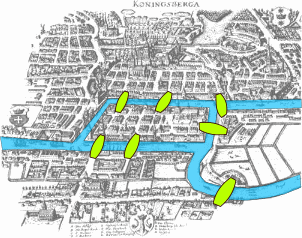
\includegraphics{Konigsberg_bridges.png}
\caption{Konigsberg in Euler's time}
\end{figure}

A group of friends enjoyed strolling through the city, and created a
game: could they take a walk in the city, crossing every bridge exactly
once, and return to where they started from? Eventually, Euler proved
that such a walk is not possible, and in doing so founded graph theory.

\subsubsection{Eulerian Cycles}\label{eulerian-cycles}

Before presenting Euler's proof, let us formulate the question precisely
in terms of graph theory, which will also generalize the problem.

We can produce a graph \(\Gamma_K\), which we will callt he Kingsberg
graph, that represents the city of Konigsberg as follows. There will be
four vertices, representing the four land-masses are vertices. Every
bridge will be represented by an edge.

Then, the question reduces to finding a closed walk in the graph that
will uses every edge exactly once. In particular, this walk will not use
any edge more than once and hence will be a trail (though it may repeat
vertices).

\subsection{Definition: Eulerian cycle}\label{definition-eulerian-cycle}

Let \(\Gamma\) be any graph. An \emph{Eulerian cycle} or \emph{Eulerian
tour} is a walk in \(\Gamma\) that visits every edge exactly once.

The citizens Konigsberg were asking whether an Eulerian cycle existed in
\(\Gamma_K\). Euler did more: he gave simple criterion to tell whether
or not \emph{any} connected graph \(\Gamma\) has an Eulerian tour. We
will now state and prove his result.

\subsection{Theorem}\label{theorem}

A connected graph \(\Gamma\) (without loops) has an Eulerian cycle if
and only if every vertex of \(\Gamma\) has even degree.

\subsection{Proof}\label{proof-3}

First, we show this condition is necessary. Let \(\Gamma\) be a
connected graph, and suppose that it has an Eulerian cycle
\(w=v_0, e_1, v_1,\dots, e_n, v_n\). Let \(v\) be any vertex in
\(\Gamma\); we must show that \(v\) has even degree. We will do this by
pairing up the edges incident to \(v\).

Since \(w\) is a closed walked, we may assume that it does not start at
\(v\). Then consider the first time that the walk \(w\) visits \(v\) --
it will enter by some edge \(e_i\), and leave by some other edge
\(e_{i+1}\). We pair these two edges up.

The walk \(w\) may visit \(v\) multiple times; each time it does, it
must enter from one edge, and leave from another edge. Each time the
walk \(w\) visits \(e\), we will pair up the edge the walk \(w\) entered
with the edge \(w\) left by. Since by supposition the walk \(w\) uses
every edge of \(\Gamma\) exactly once, we see that every edge incident
to \(v\) will be paired up with exactly one other edge in this way, and
hence \(v\) must have even degree.

We now show that this condition is sufficient. That is, we suppose that
every vertex of \(\Gamma\) has even degree; we must show that \(\Gamma\)
has an Eulerian cycle. We will proceed by induction on the number of
edges of \(\Gamma\).

Any connected graph with 0 edges consists of just a vertex, and hence
trivially has an Eulerian cycle.

Now, for the inductive step, we suppose that \(\Gamma\) has \(n\) edges,
and further suppose that we know Euler's theorem is true for all graphs
with less than \(n\) edges -- that is, suppose that every connected
graph \(\Gamma\) with less than \(n\) edges, all of whose vertices have
even degree has an Eulerian walk.

We first claim that \(\Gamma\) has \emph{some} closed trail. Start at
any vertex \(v_0\). Since \(\Gamma\) is connected, \(v_0\) has at least
one edge \(e_1\) so we start our trail with \(v_0, e_1, v_1\). Since
every vertex has an even degree, there must be another edge out of
\(v_1\), say \(e_2\) leading to \(v_2\).

We continue building a trail in \(\Gamma\) by randomly selecting an
unused edge of \(\Gamma\) at our current vertex. Since every vertex has
even degree, and whenever our trail visits a vertex we use up edges two
at a time (coming and going), we see that whenever we arrive at a vertex
\(v\), there must be another edge leaving it to continue our trail --
unless perhaps we hit our starting vertex \(v_0\), where we have only
used one edge up. Thus, if we randomly start building a trail we must
eventually return to our starting vertex and obtain a closed trail.

Now, given our graph \(\Gamma\), we know it has \emph{some} closed trail
\(w\). If \(w\) uses every edge of \(\Gamma\), we are done. If not, we
consider the new graph \(\Gamma^\prime\) obtained by deleting every edge
of \(w\) (but not the vertices). Note that every vertex of
\(\Gamma^\prime\) has even degree. Second, \(\Gamma^\prime\) may not be
connected, but each connected component \(\Gamma_i^\prime\) of
\(\Gamma^\prime\) has fewer edges that \(\Gamma\) and hence has an
Eulerian tour \(u_i\) by supposition. Together, \(w\) and the \(u_i\)
visit every edge of \(\Gamma\) exactly once. We can stitch them together
into one closed path as follows -- each \(u_i\) shares at least one
vertex \(v_i\) with \(w\). We trace the path \(w\), but the first time
we visit vertex \(v_i\) we insert the path \(u_i\) before continuing
along \(w\). \(\square\)

\section{Lecture 5: Hamiltonian cycles}

\subsection{Definition}\label{definition-2}

A graph \(\Gamma\) is \emph{Hamilton} if there exists a closed walk that
visits every vertex exactly once.

Although the definition of a Hamiltonian graph is extremely similar to
an Eulerian graph, it is much harder to determine whether a graph is
Hamiltonian or not: doing so is an NP-complete problem.

\subsection{Examples}\label{examples-1}

\subsection{Proposition}\label{proposition}

The Petersen graph is \emph{not} Hamiltonian.

\subsection{Proof}\label{proof-4}

Suppose the Petersen graph was Hamiltonian, and let
\(v_0-v_1-v_2-v_3-\cdots-v_{9}-v_0\) denote the Hamiltonian cycle, as we
have drawn below:

The Petersen graph has 15 edges, and the Hamiltonian cycle uses 10 of
them, so there must be 5 edges left in the Petersen graph that are not
in the Hamiltonian cycle. The proof works by considering the
possibilities for these 5 extra edges.

Let us consider the extra edge incident to \(v_0\); the others are
equivalent. Since the Petersen graph has no loops or multiple edges,
this edge cannot go from \(v_0\) to itself, or to \(v_1\) or \(v_9\).

Since the Petersen graph has no triangles or 4 cycles, this edge cannot
``skip'' 1 or 2 vertices in the Hamiltonian cycle. More specifically, we
cannot we cannot have an edge from \(v_0\) to \(v_2\) or \(v_8\), as
these make triangles, as in the dashed edges below:

And we cannot have edges \(v_0\) to \(v_3\) or to \(v_7\), as these make
4 cycles:

Thus, the only possibility for these edges is that they ``skip'' 4 or 5
vertices (skipping more than 5 vertices is the same as skipping less
vertices in the other direction). So for instance, \(v_0\) can only be
connected to \(v_4, v_5\) or \(v_6\) with its extra edge.

We now claim that at least one of these extra edges must ``skip'' 4
vertices. If not, then every extra edge would skip 5 vertices. Since
each vertex has degree 3, there must be one extra edge through each of
these vertices, connecting to the opposite vertex. But this
configuration has many four cycles -- for instance,
\(v_0-v_1-v_6-v_5-v_0\). Since the Petersen graph does not have any 4
cycles, we see this cannot occur:

Relabeling our edges if necesary, we can make the extra edge that skips
the 4 cycle be the edge \(v_0-v_4\). Now, consider the extra edge at
\(v_5\). This cannot skip 5, because that would make it adjacent to
\(v_0\), which already has its extra edge. Thus, it must skip 4, and be
adjacent to either \(v_9\) or \(v_1\). But since each of these are
adjacent to \(v_0\), it would create a 4-cycle: either
\(v_0-v_4-v_5-v_9-v_0\), or \(v_0-v_4-v_5-v_1-v_0\).

We have drawn the edge from \(v_0\) to \(v_4\) in solid red; any of the
dashed edges from \(v_5\) create a configuration not found in the
Petersen graph:

\(\square\)

\subsubsection{Partial results on Hamiltonian
graphs}\label{partial-results-on-hamiltonian-graphs}

Although there is no complete characterisation of Hamiltonian graphs,
there are several nice sufficient conditions for a graph to be
Hamiltonian;

\subsection{Ore's Theorem}\label{ores-theorem}

Let \(\Gamma\) be a simple graph with \(n\) vertices such that for any
two nonadjacent vertices \(v\) and \(w\), we have
\(\text{deg}(v)+\deg{w}\geq n\). Then \(\Gamma\) is Hamiltonian.

\subsection{Proof}\label{proof-5}

We will give a proof by contradiction. First, suppose that \(\Gamma\)
were a counterexample. Adding edges to \(\Gamma\) preserves the
condition on the degrees, and so we may continually add edges to
\(\Gamma\) until adding any more would create a Hamiltonian cycle. We
will thus assume that \(\Gamma\) is a counterexample with the maximal
set of edges.

The benefit of this is that such a \(\Gamma\) must have a non-closed
path that visits every vertex exactly once. To see this, add one more
edge \(e\) to \(\Gamma\) -- the resulting graph then has a Hamiltonian
cycle, which must pass through \(e\), deleting \(e\) give the desired
path.

Let \(v_1-v_2-\dots v_{n-1}-v_n\) be the path visiting every vertex of
\(\Gamma\). We will complete the proof by showing there exists an
\(i\in 3,\cdots, n-1\) so that \(v_1\) is adjacent to \(v_i\) and
\(v_n\) is adjacent to \(v_{i-1}\). This completes the proof because
\(v_1-v_2-\cdots v_{i-1}-v_n-v_{n-1}-v_{n-2}-\dots v_i-v_1\) is a
Hamiltonian path. We illustrate this below, with \(n=9\) and \(i=5\):

The existence of such an \(i\) follows from the pigeon hole principle.
Since \(v_1\) and \(v_n\) are not adjacent by supposition, the sum of
their degrees is at least \(n\). Two edges incident to them are
accounted for \(v_1-v_2\), and \(v_{n-1}-v_{n-2}\), so there must be at
least \(n-2\) other edges incident to \(v_1\) or \(v_{n}\). Since
\(\Gamma\) is simple, any such edge out of \(v_1\) has \(n-3\)
possibilities: \(v_3, v_4, \dots, v_{n-1}\). Similarly, there are
\(n-3\) possibilities for an edge adjacent to \(v_n\) --
\(v_2,v_3,\dots, v_{n-2}\). We pair these edges up into the
possibilities we want, creating \(n-3\) bins. Since there are \(n-2\)
edges we need to distribute among these bins, one of the bins must
contain at least two, which is exactly what we needed to show.

\section{Lecture 6: Trees}

\subsection{Definition}\label{definition-3}

A \emph{forest} is a graph with no cycles; a \emph{tree} is a connected
graph with no nontrivial closed trails.

Thus, a forest is a disjoint union of trees.

\subsection{Example}\label{example-1}

The following graph is a forest consisting of three trees:

\begin{figure}[htbp]
\centering
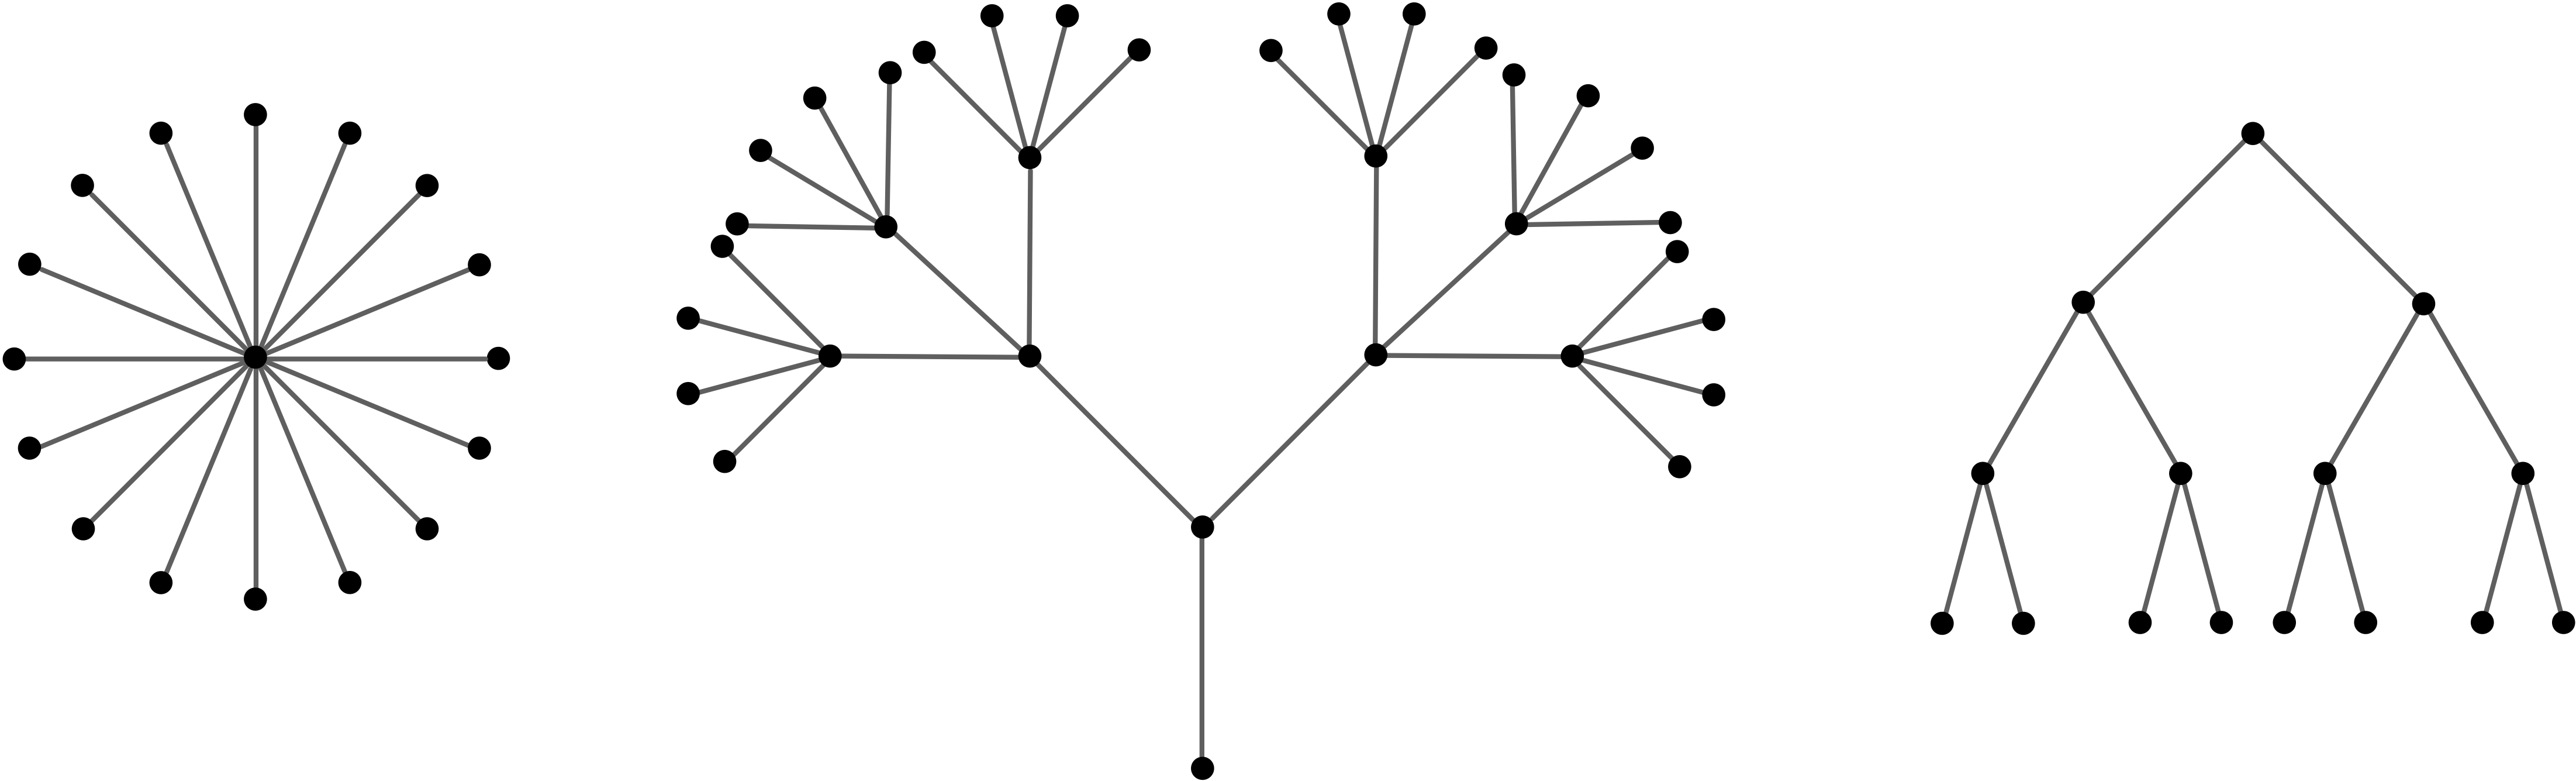
\includegraphics{../Slides/Pictures/forest.png}
\caption{A small forest}
\end{figure}

The following graph is a \emph{not} a tree:

\begin{figure}[htbp]
\centering
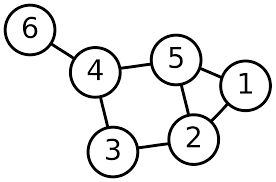
\includegraphics{../Slides/Pictures/notatree.png}
\caption{Not a graph}
\end{figure}

Consider the two conditions of being tree: being connected, and not
having any cycles.

The first condition is somehow saying that \(\Gamma\) has \emph{enough}
edges: to be connected, we need a path between any two vertices, and the
more edges we have, the more likely this is to happen.

The second condition is somehow saying that \(\Gamma\) doesn't have
\emph{too many} edges: we \emph{don't} want cycles, and having more
edges makes that more likely.

Thus, being a tree a bit of a goldilocks condition -- it has \emph{just
the right} amount of edges. It's not \emph{just} how many edges the
graph has, though -- the path graph \(P_4\) has 4 vertices and 3 edges,
and is a tree, but the disjoint union of a triangle and a single vertex
also has 4 vertices and 3 edges but is not a tree.

The following proposition summarises this discussion and makes it more
precise:

\subsection{Proposition}\label{proposition-1}

Let \(\Gamma\) be a graph with \(n\) vertices. The following are
equivalent:

\begin{enumerate}
\def\labelenumi{\arabic{enumi}.}
\tightlist
\item
  \(\Gamma\) is a tree.
\item
  Between any two vertices \(a,b\in V(\Gamma)\), there is a unique path.
\item
  \(\Gamma\) is connected, but removing any edge makes \(\Gamma\)
  disconnected.
\item
  \(\Gamma\) has no cycles, but adding any edges to \(\Gamma\) creates a
  cycle.
\item
  \(\Gamma\) is connected and has \(n-1\) edges
\item
  \(\Gamma\) has no cycles and has \(n-1\) edges
\end{enumerate}

\subsubsection{Proof:}\label{proof-6}

We will not show all of the equivalences. Some are tricky to do
directly; a few we will put on the practice sheet.

\subsection{1 implies 3}\label{implies-3}

Trees are by definition connected, so we must show that removing any
edge of \(\Gamma\) disconnects \(\Gamma\). Let \(a\) and \(b\) be two
adjacent vertices, and suppose removing the edge between them did not
disconnect \(\Gamma\). Then there is a path from \(a\) to \(b\) in
\(\Gamma\) not using the edge connecting them; adding the last edge back
in makes a cycle, a condtradiction.

\subsection{3 implies 2}\label{implies-2}

Since \(\Gamma\) is connected, there is at least one path between two
vertices. If there were two paths between \(a\) and \(b\), then deleting
any edge \(e\) that was only in one of the paths wouldn't disconnected
\(\Gamma\).

\subsection{2 implies 1}\label{implies-1}

Suppose that \(\Gamma\) is a graph with a unique path between any two
vertices. Then, in particular \(\Gamma\) is connected, and so to show
\(\Gamma\) is a tree we must show it has no cycles.

Suppose \(v_0, e_1, v_1,\dots, e_n, v_n=v_0\) was a cycle in \(\Gamma\).
Then there are two paths between \(v_0\) and \(v_1\) -- the edge
\(e_1\), or the path \(v_1, e_2, v_2,\dots, v_n=v_0\). This is a
contradiction, and hence \(\Gamma\) has no cycles.

We will also show that if \(\Gamma\) is a tree with \(n\) vertices, then
\(\Gamma\) has \(n-1\) edges. Since we know trees are connected and have
no cycles, this means any of 1-3 imply 5 and 6.

We proceed by induction: the proof is obvious when \(n\) is one or two
-- a tree on one vertex has no edges, and a tree on two vertices has a
single edge. Thus, we have a base case.

We now assume that all trees with at most \(k\) vertices have \(k-1\)
edges for all \(k<n\) and we must show that a tree with \(n\) vertices
has \(n-1\) edges. Pick any edge \(e\) of \(\Gamma\) are remove it. By
3, the result \(\Gamma\setminus e\) is disconnected.

We claim that \(\Gamma\setminus e\) consists of exactly two connected
components. Pick any two vertices \(a,b\in\Gamma\). By 2, there is a
unique path between them; if that path contains \(e\), there will be no
path between \(a, b\) in \(\Gamma\setminus e\), and hence they must lie
in different components of \(\Gamma\setminus e\). If the path between
\(a\) and \(b\) does not contain \(e\), then they will lie in the same
component. Hence, if \(v, w\) are the two ends of the edge \(e\), then
every vertex of \(\Gamma\setminus e\) has a path to either \(v\) or
\(w\), but not both.

Thus, we see \(\Gamma\setminus e\) has two components \(G_1\) and
\(G_2\), each of which are trees: they are connected, and have no
cycles. Suppose \(G_1\) contain \(k\) vertices; then \(G_2\) must have
\(n-k\) vertices. By the inductive hypothesis, we know they must contain
\(k-1\) edges and \(n-k-1\) edges respectively.

\subsubsection{\texorpdfstring{The edges in \(\Gamma\) are \(e\) and the
edges of \(G_1\) and \(G_2\), hence we see that \(\Gamma\) has
\(1+(k-1)+(n-k-1)=n-1\) edges, as
desired.}{The edges in \textbackslash{}Gamma are e and the edges of G\_1 and G\_2, hence we see that \textbackslash{}Gamma has 1+(k-1)+(n-k-1)=n-1 edges, as desired.}}\label{the-edges-in-gamma-are-e-and-the-edges-of-gux5f1-and-gux5f2-hence-we-see-that-gamma-has-1k-1n-k-1n-1-edges-as-desired.}

\section{The Lost Lecture 7: Leaves, chemistry, spanning trees comments} 

Note: This lecture didn't happen because I was ill; the material
presented here either has gotten absorbed into other lectures or problem
sets, or won't be examined; I leave it here for completeness.

A useful concept when studying trees is that of a leaf:

\subsection{Definition}\label{definition-4}

A \emph{leaf} in a tree is a vertex of degree 1.

\subsection{Lemma}\label{lemma-2}

Every finite tree with at least two vertices has at least two leaves.

\subsection{Lemma}\label{lemma-3}

Every finite tree with at least two vertices has at least two leaves.

\subsection{Proof 1: using paths}\label{proof-1-using-paths}

Suppose \(T\) is at tree. Since \(T\) has at least two vertices, at has
at least one edge. Pick any edge \(e\), say, between \(a\) and \(b\). If
the vertex \(a\) is a leaf, we have at least one leaf. If not, there is
another edge incident to \(a\). and we can start a path from \(a\) away
from \(e\) following this edge. As long as the end vertex of our path is
not a leaf we may continue our path, and we will never return to a
vertex we have already encountered, since trees have unique paths
between vertices. Since \(T\) is finite, the path must eventually
terminate -- i.e., find a leaf.

Following the same argument from the vertex \(b\) produces another leaf.
\(\square\)

\subsection{Proof 2: using handshaking}\label{proof-2-using-handshaking}

We will use that \(\Gamma\) is connected, has \(n>2\) vertices, and
\(n-1\) edges.

Since \(\Gamma\) is a tree it is connected; since it has connected and
has two vertices it cannot have any vertices of degree 0.

Thus, if we assume for a contradiction that \(\Gamma\) has no leaves,
then every vertex \(\Gamma\) had degree at least two. Since we know
\(\Gamma\) has \(n\) vertices and \(n-1\) leaves, applying the
handshaking lemma gives:

\[2n-2=2 |E(\Gamma)|=\sum_{v\in V(\Gamma)} d(v)\geq \sum_{v\in V(\Gamma)} 2=2n\]
a contradiction. For the inequality to hold, \(\Gamma\] must have at
least two vertices of degree 1. \(\square\]

Leaves will play a very important role in this afternoon's lecture on
the Prüfer code. In the meantime, we point out that the handshaking
argument we give another application of the handshaking lemma argument
above. Recall that in the last lecture we stated the following, but did
not provide a full proof:

\subsection{Proposition}\label{proposition-2}

Let \(\Gamma\) be a graph with \(n\) vertices. The following are
equivalent:

\begin{enumerate}
\def\labelenumi{\arabic{enumi}.}
\tightlist
\item
  \(\Gamma\) is a tree.
\item
  Between any two vertices \(a,b\in V(\Gamma)\), there is a unique path.
\item
  \(\Gamma\) is connected, but removing any edge makes \(\Gamma\)
  disconnected.
\item
  \(\Gamma\) has no cycles, but adding any edges to \(\Gamma\) creates a
  cycle.
\item
  \(\Gamma\) is connected and has \(n-1\) edges
\item
  \(\Gamma\) has no cycles and has \(n-1\) edges
\end{enumerate}

In lecture we showed that 1-3 are equivalent, and that if \(\Gamma\) is
a tree with \(n\) vertices, then \(\Gamma\) has \(n-1\) edges, and hence
that any of 1-3 imply 5 and 6. Today we are going to use that 5 implies
1, hence we will prove it.

\subsection{Lemma}\label{lemma-4}

Suppose that \(\Gamma\) is connected and has \(n\) vertices and \(n-1\)
edges. Then \(\Gamma\) is a tree.

\subsection{Proof}\label{proof-7}

We will use induction. As a base case, the result is clear if \(n\) is 1
or 2. Thus, we assume that all connected graphs with \(k<n\) vertices
and \(k-1\) edge are trees, and we must show that if \(\Gamma\) is
connected and has \(n-1\) edges, then \(\Gamma\) is a tree.

Note that \(\Gamma\) has at least two vertices of degree 1, as the
handshaking lemma argument given above only uses the facts that
\(\Gamma\) is connected and has the right number of leaves.

Now suppose that \(v\in \Gamma\) has degree one, and let \(e\) be the
edge incident to \(v\). Let \(\Gamma^\prime\) be the graph obtained by
removing \(v\) and \(e\). Then \(\Gamma^\prime\) has \(n-1\) vertices
and \(n-2\) edges. Further, since \(\Gamma\) was connected, we see that
\(\Gamma^\prime\) is as well. Thus, by the inductive hypothesis,
\(\Gamma^\prime\) is a tree, and so \(\Gamma\) is as well

\subsubsection{Chemistry Application:
Alkanes}\label{chemistry-application-alkanes}

In organic chemistry, an \emph{alkane} is a molecule with formula
\(C_nH_{2n+2}\). The simplest Alkanes are methane \(CH_4\), ethane
\(C_2H_6\) and propane \(C_3H_8\).

\begin{figure}[htbp]
\centering
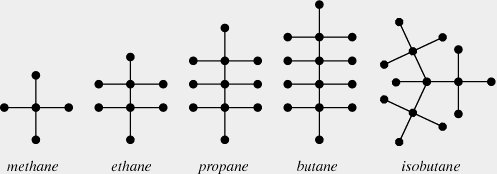
\includegraphics{../Slides/Pictures/Hydrocarbons.jpg}
\caption{Alkanes}
\end{figure}

It appears from the graph that Alkanes are all trees; we prove that now.

\subsection{Lemma}\label{lemma-5}

Any alkane \(C_nH_{2n+2}\) is a tree.

\subsection{Proof}\label{proof-8}

We will use that a connected graphs on \(m\) vertices with \(m-1\) edges
is a tree.

Any graph of a molecule is necessarily connected, and so to prove an
Alkane is a tree we must count the number of vertices and edges.

There are \(n+(2n+2)=3n+2\) vertices.

We count the edges using the Handshaking lemma. Carbon atoms have
valency 4, and there are \(n\) of them, while Hydrogen atoms have
valency 1. Thus, the sum of all the degrees of the vertices is \(6n+2\).
The number of edges is half of these, namely \(3n+1\), which is 1 less
than the number of vertices. Since to be an atom it must be connected,
we see that any Alkane is a tree. \(\square\)

\subsubsection{Isomers}\label{isomers}

\subsection{Definition}\label{definition-5}

Two molecules are \emph{isomers} if they have the same molecular
formula, but the molecules are put together in a different way.

When there are 1, 2 or 3 carbon molecules, the only possible Alkanes is
a line of carbon molecules. The resulting chemicals are methane, ethane,
and propane. when \(n=4\), there are two possible alignments of the
Carbon atoms: in a line, which is butane, or in a `T' shape, which is
isobutane; when \(n=5\), there are three different possibilities.

Around 1875, Hamilton used graph theory to count the number of isomers
of the Alkane \(C_nH_{2n+2}\). One can forget about the placement of the
hydrogen molecules, and just count the struture of the carbon molecules;
these two will be a tree. Since the valency of Carbon is four the
maximum degree of a vertex in these trees will be 4, and so counting
isomers of \(C_nH_{2n+2}\) is equivalent to counting isomorphism classes
of trees with \(n\) vertices, all of degree at most 4.

\section{Lecture 8: Prüfer code}

In this lecture, we will prove Cayley's formula, using the Prüfer code.
In particular, we will give a map \(PC\) that takes in a labelled tree
with \(n\) vertices, and returns a string of \(n-2\) numbers, each
between \(1\) and \(n\), and an inverse map \(\mathbf{Tree}\) that takes
in a string of numbers and returns a labelled tree.

The starting observation is that to write down a labelled tree is the
same as writing down its \(n-1\) edges. Since the vertices are ordered,
each edge can be written down by a pair of numbers in
\(\{1,\dots,n \}\). The Prüfer code begins by writing down these edges
in a clever ordering.

\subsubsection{The Prüfer code}\label{the-pruxfcfer-code}

We are now ready to introduce the Prüfer code. We begin by writing down
the edges of \(T\). The two vertices of each edge will be written down
in a column, with the parent vertex in the top row and the child vertex
on the bottom row. We record the edges in the following specific order.

First, find the lowest numbered leaf, and record its number in the
bottom row. Above it, write down the number of the vertex this leaf is
adjacent to, which we call the parent vertex. Now, delete that lowest
numbered leaf and the edge connecting it to the rest of the tree. Find
the lowest leaf on the resulting vertex, and record its number, and the
number of its parent, in the next column.

Iterate this procedure until we have written down all \(n-1\) edges of
our tree, with the leaf numbers in the top row, and the parent numbers
in the bottom row.

The list of the first \(n-2\) parent numbers (i.e., all but the last),
is the Prüfer code of \(T\).

\subsection{Example}\label{example-2}

We illustrate the construction of the Prüfer code by finding the code
for the following labelled tree:

The lowest leaf is 3, which is attached to 1, so the first column goes

\begin{tabular}{c c c c c c c}
  Parent node & 1 & 6 & 6 & 2 & 2 & 7 \\
  Child node & 3 & 1 & 4 & 5 & 6 & 2
\end{tabular}

Thus, the Prüfer code for the above tree is 16622.

\subsection{Reconstructing a tree from its Prüfer
Code}\label{reconstructing-a-tree-from-its-pruxfcfer-code}

It is clear from the above definition that the Prüfer code is a list of
\(n-2\) numbers between 1 and \(n\); it is not clear that any such list
of numbers is obtained, nor that any two trees give us a different set
of numbers. To see this, we describe an inverse algorithm, that
constructs a tree on \(n\) vertices from a Prüfer code.

More explicitly, the inverse algorithm will take as input a Prüfer code,
and from that Prüfer code it will reconstruct the full ordered table of
edges we constructed in the Prüfer code algorithm. It should be clear
from the description that the algorithm actually reproduces this table,
and not some other table, and hence that the two algorithms are inverse
to each other. This shows that the Prüfer code is a bijection, which
proves Cayley's formula, as there are \(n^{n-2}\) valid Prüfer codes on
\(n\) vertices.

This algorith proceeds by figuring out the corresponding child nodes one
by one. Recall that any number in our list appeared as a parent node,
and so is not a leaf. At the first step, we deleted the smallest leaf.
So the first child node is the smallest number that does not appear on
our list.

After we recorded that edge, we deleted it; thus, the second child
number is the smallest number that we haven't

\begin{enumerate}
\def\labelenumi{\arabic{enumi}.}
\tightlist
\item
  already used as a leaf number\\
\item
  doesn't appear at or after the current spot as a parent.
\end{enumerate}

\subsection{Example}\label{example-3}

We first reconstruct the tree we did in the first example, from its
code. Recall, the Prüfer code was 1 6 6 2 2.

The lowest unused number is 3, so that is the first child.

To find the next unused number, we move to the second column. 1 only
appears in the first column, and so it is now the lowest number that
doesn't appear, and so it goes underneath the first 6. Moving to the
third column, we have already used 1 and 3 as child nodes. The number 2
is still to appear as a parent, and so can't be a leaf yet, and so 4 is
the first number that we haven't used yet. Similar reasoning gives 5 and
7 for the 4th and 5th column.

Finally, the last remaining edge connects the two nodes we have not used
as leaves yet; in this case 2 and 6.

\subsubsection{Number of trees with a given degree
sequence}\label{number-of-trees-with-a-given-degree-sequence}

The Prüfer code actually proves a stronger statement: it counts the
number of labelled trees where vertex \(i\) has degree \(d_i\). More
specifically:

\subsection{Corollary}\label{corollary}

The number of labelled trees on \(n\) vertices where vertex \(i\) has
degree \(d_i\) is

\[\left( \begin{array}{cc} n-2 \\ d_1-1,d_2-1,\dots, d_n-1 \end{array}\right)=\frac{(n-2)!}{(d_1-1)!(d_2-1)!\cdots (d_n-1)!}\]

\subsection{Proof}\label{proof-9}

First, observe that vertex \(i\) of a labeled tree \(T\) has degree
\(d_i\) if and only if \(i\) appears \(d_i-1\) times in the Prüfer code
\(PC(T)\). This can be seen by building the Prüfer code: each time \(i\)
occurs in the Prüfer code we delete an edge incident to \(i\), and
finally \(i\) will occur a final time as a leaf.

Then, the number of labeled trees we want to count is the number of
sequences of \(n-2\) numbers, where \(i\) occurs \(d_i-1\) times, which
is counted by the given multinomial coefficient.

\section{Lecture 9: Spanning Trees, Kruskal's algorithm}

\subsubsection{Spanning trees}\label{spanning-trees}

\subsection{Definition}\label{definition-6}

Let \(\Gamma\) be a graph. A \emph{spanning tree} of \(\Gamma\) is a
subgraph \(T\subset \Gamma\) such that \(T\) is a tree and \(T\)
contains every vertex of \(\Gamma\).

Spanning trees are useful because they are a minimal connected subgraph
that lets us get to all of \(\Gamma\). For instance, if the vertices are
cities and the edges are roads, a spanning tree is a minimal set of
edges that guarantee that you can get from any one city to another.

\subsection{Examples:}\label{examples-2}

\begin{itemize}
\item
  The cycle graph \(C_n\) has \(n\) spanning trees obtained by deleting
  any one edge.
\item
  A spanning tree of the complete graph \(K_n\) is the same thing as a
  labelled tree, so there are \(n^{n-2}\) such spanning trees by
  Cayley's theorem.
\end{itemize}

\subsection{Lemma:}\label{lemma-6}

Every connected graph \(\Gamma\) has a spanning tree.

\subsection{Proof}\label{proof-10}

By our characterisation of trees, if \(T\) is connected and has no
cycles, then \(T\) is a tree. So it is enough to find a connected
subgraph \(T\) of \(\Gamma\) that contains every vertex.

Let \(H\) be any subgraph of \(\Gamma\) that is connected and contains
all the vertices of \(\Gamma\). If \(H\) has a cycle, we can pick any
edge \(e\) of that cycle and delete it, and \(H\) will still be
connected: any path that used \(e\) can use the rest of the cycle
instead.

Thus, starting from \(\Gamma\), we may repeatedly remove edges from
cycles and not disconnect \(\Gamma\) until there are no more cycles
left; the result will be a spanning tree. \(\square\)

\subsubsection{Introduction to optimisation
problems}\label{introduction-to-optimisation-problems}

One motivation for introducing trees was as the ``cheapest'' way of
connecting \(n\) points. Here, ``cheapest'' just means the least number
of edges. In real world applications, not all edges are created equal.
For example, consider the case where the vertices of \(\Gamma\)
represent cities, and the edges are roads connecting them. If we're
looking for the shortest path between two cities, we do not just want
the least number of edges, as some roads will be longer than others, or
be busy and take longer to drive. These subtleties can be addressed with
a \emph{weighted graph}.

\subsection{Definition}\label{definition-7}

A \emph{weighted graph} is a graph \(\Gamma\), together with a
non-negative real number \(w(e)\) for each edge \(e\in E(\Gamma)\).

\subsection{Example}\label{example-4}

Typically, weighted graphs are presented by drawing labelling each edge
of the graph with its weight:

\begin{figure}[htbp]
\centering
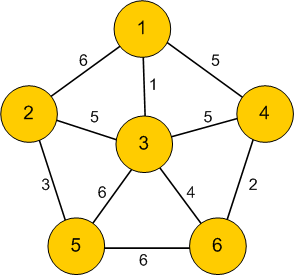
\includegraphics{../Slides/Pictures/weightedgraph.png}
\caption{Example of a weighted graph}
\end{figure}

\subsection{Real world examples of
weights}\label{real-world-examples-of-weights}

Even in the case where the vertices of \(\Gamma\) are cities and the
edges are conenctions between them, there are many possible
interpretations of edges weights: - The edge weights \(w(e)\) might
represent the cost of building or maintaining the road between the city
- The edge weights migth represent the distance between the cities - The
edge weights might represent travel times between the cities - the edge
weights might represent the cost of a train/plane ticket between the
cities

In the next few class lectures, we will discuss the following
optimisation problems for weighted graphs:

\begin{itemize}
\tightlist
\item
  The \emph{minimal spanning tree} -- finding a spanning tree \(T\) of
  \(\Gamma\) where the total cost of the edges in \(T\) is the cheapest
  among all spanning trees of \(\Gamma\).
\item
  The \emph{shortest path} -- finding a path between two vertices of
  \(\Gamma\), where the total weight of all the edges in the path is
  minimal among all paths between the two vertices.
\item
  The \emph{traveling salesman problem} -- finding a hamiltonian cycle
  in a graph \(\Gamma\) where the total weight of all the edges is
  minimal.
\end{itemize}

\subsubsection{Kruskal's algorithm}\label{kruskals-algorithm}

We now present Kruskal's algorithm, which solves the problem of finding
a minimal weight spanning tree in a weighted graph \(\Gamma\). Before
discussing the algorithn, let's look at a toy example to get an idea of
the problem.

\subsection{Example}\label{example-5}

Consider the following weighted graph:

Obviously, there are three spanning trees, obtained by removing one of
the three edges. The spanning tree A-B-C has weight 7, B-C-A has weight
6, C-A-B has weight 5, and so we have found the cheapest spanning tree.

Any finite graph will only have finitely many spanning trees, and so it
is always possible to exhaustively find all of them, compute their
weights, and hence find the cheapest. However, for large graphs there
will be many spanning trees. For example, a spanning tree of the
complete graph \(K_n\) is equivalent to a labelled tree on \(n\)
vertices, and by Cayley we know there are \(n^{n-2}\) of these trees,
which grows faster than exponential or factorial! Thus, in practice, to
find a minimal spanning tree we need a more efficient algorithm than
brute forst checking all the possibilities.

\subsection{Kruskal's algorthm}\label{kruskals-algorthm}

For finding spanning trees, it turns out there are several easy
algorithms that will always find the cheapest spanning tree. Many of
them are \emph{greedy algorithms}, which do not ``plan ahead'', but
rather blindly do the best possible next step. Kruskal's algorithm is an
example of these, which builds a spanning tree \(T\) step by step,
starting from the subgraph of \(\Gamma\) consisting just of the vertices
of \(\Gamma\) and no edges:

\begin{enumerate}
\def\labelenumi{\arabic{enumi}.}
\tightlist
\item
  Find the cheapest edge \(e\) remaining from \(\Gamma\), and remove it
  from \(\Gamma\).
\item
  If adding \(e\) to \(T\) will not make any loops, add it to \(T\).
  Otherwise, discard it.
\item
  Iterate the first two steps until \(T\) is a spanning tree.
\end{enumerate}

In class we now ran an example of Kruskal's algorithm -- we'll skip that
in the note, but there are many such examples available online, for
instance, in this short Youtube video .

Note that to have a spanning tree, the graph \(\Gamma\) must be
connected. Running Kruskal's algorithm on a disconnected graph will
produce a spanning tree for each component of \(\Gamma\).




\subsection{Proof of the correctness of Kruskal's
algorithm:}\label{proof-of-the-correctness-of-kruskals-algorithm}

From a mathematical point of view, the interesting part is to prove that
running Kruskal's algorithm on a connected graph will always produce a
minimal spanning tree. There are two things to prove: that the end
result of Kruskal's algorithm actually is a spanning tree, and that it
is a minimal cost spanning tree. We prove the first part now, and the
second part in this afternoon's lecture.

To prove the first part, we first note that the graph \(T\) produced by
Kruskal's algorithm contains all the vertices of \(\Gamma\), as they
were all added at the beginning. Thus, we only have to show that \(T\)
is a tree -- that is, it is connected, and that it has no cycles.

Suppose that \(T\) consisted of more than one component. Since
\(\Gamma\) is connected, there would be two components of \(T\), say,
\(C_1\) and \(C_2\), with edges between \(C_1\) and \(C_2\). But adding
the cheapest such edge to \(T\) does not create any loops, and hence it
would have been added by Kruskal's algorithm, a contradiction.

It is immediate that \(T\) will not have any loops, because Kruskal's
algorithm checks to make sure no loops are created before it adds an
edge. Thus, the output of Kruskal's algorithm is always a spanning tree.

\section{Lecture 10: Kruskal proof, Traveling Salesman}

\subsection{Kruskal's completed:}\label{kruskals-completed}

In this morning's lecture we described Kruskal's algorithm for finding a
minimal weight spanning tree in a weighted graph. After demonstrating
the algorithm, we showed that it always produces a spanning tree, but we
have not yet shown that this spanning tree has minimal weight. We do
that now.

The proof will be inductive. Let \(T_0\) be the subgraph that Kruskal's
algorithm starts with, namely, all the vertices of \(\Gamma\) and none
of the edges. Let \(T_k\subset\Gamma\) be the subgraph Kruskal's
produces after adding \(k\) edges to \(T_0\). We willinductively prove
that \(T_k\) is contained in \emph{some} minimal spanning tree of
\(\Gamma\). In particular, since we know \(T_{n-1}\) is a spanning tree,
we see that \(T_{n-1}\) will be a minimal weight spanning tree.

The base case is clear: any minimal spanning tree contains all the
vertices of \(\Gamma\), which is the initial graph \(T_0\), and since
\(\Gamma\) is finite there exists \emph{some} minimal spanning tree.

For the inductive step, we assume that \(T_k\) produced from Kruskal's
algorithm is contained in some minimal spanning tree \(M\), and
Kruskal's algorithm tells us we should construct \(T_{k+1}\) from
\(T_k\) by adding the edge \(e\) to \(T\). We need to prove that
\(T_{k+1}\) is contained in some minimal weight spanning tree
\(M^\prime\). We claim we can take
\(M^\prime=M\setminus\{e\}\cup\{f\}\).

First, note that \(M^\prime\) is indeed a spanning tree; since
\(M\cup e\) has a cycle, \(M^\prime\) is connected, and it has the right
number of edges.

Now, we must show \(M^\prime\) has minimal weight. Since \(M^\prime\)
only differs from \(M\) (which had minimal weight) by adding \(f\) and
removing \(e\), we see that \(w(M^\prime)=w(M)\) if and only if
\(w(e)=w(f)\).

Since \(M\) is by supposition a minimal weight spanning tree, we have
that \(w(f)\leq w(e)\). Since Kruskal's algorithm is trying to add the
edge \(e\) instead of \(f\), we have that either \(w(e)\leq w(f)\), or
that adding \(f\) to \(T\) creates a cycle. But
\(T\cup f\subset M^\prime\) which is a tree, so it cannot be creating a
cycle, and we must have that \(w(e)\leq w(f)\).

Thus, \(w(e)=w(f)\), and so \(M^\prime\) is a minimal weight spanning
tree that contains \(T\cup e.  \square\)

\subsection{Comments on minimal spanning
trees}\label{comments-on-minimal-spanning-trees}

Although Kruskal's algorithm only finds a single minimal spanning tree,
the only time Kruskal's algorithm has any choice is in what order to add
edges with the same weight. Thus, it is possible to find all minimal
spanning trees by analyzing what happens when we had a choice of edges
to add.

There are several other algorithms for finding minimal spanning trees:

\begin{enumerate}
\def\labelenumi{\arabic{enumi}.}
\tightlist
\item
  \href{https://en.wikipedia.org/wiki/Prim\%27s_algorithm}{Prim's
  algorithm} is very similar to Kruskal's algorithm, but we start from a
  single vertex, and always add the cheapest edge that is connected to
  what we already have and doesn't create any loops.
\item
  The
  \href{https://en.wikipedia.org/wiki/Reverse-delete_algorithm}{Reverse-delete
  algorithm} is the opposite of the greedy algorithm. Rather than adding
  the cheapest edge possible, the Reverse-delete algorithm worries about
  getting ``stuck'' having to add an expensive edge. It continually
  finds the most expensive edge. If removing that edge does not
  disconnect the graph, it does so. If it does disconnect the graph, it
  keeps that edge as part of the spanning tree, and finds the next most
  expensive edge.
\end{enumerate}

\subsubsection{Traveling Salesman
Problem}\label{traveling-salesman-problem}

The \emph{Traveling Salesman Problem}, abbreviated TSP, is the
following: given a weighted graph \(\Gamma\), find the cheapest
Hamiltonian path; that is, the cheapest closed walk on \(\Gamma\) that
visits every vertex exactly once.

We begin with some basic observations:

\begin{itemize}
\item
  It is enough to consider the complete graph \(K_n\). If we are given
  some other weighted graph \(\Gamma\), we can add all the edges not in
  \(\Gamma\) but make their weights \emph{much} larger than any of the
  weights inside \(\Gamma\).
\item
  The problem of determining whether a given graph \(\Gamma\) has a
  Hamiltonian cycle is a special case of the traveling salesman problem.
  To see this, suppose we're given a graph \(\Gamma\), and we want to
  determine whether it is Hamiltonian. We create a weighted \(K_n\),
  with vertices the vertices of \(\Gamma\) by giving the edge \(v-w\) a
  very small weight \(\epsilon\) if \(v\) and \(w\) \emph{are} adjacent
  in \(\Gamma\), and a very large weight \(M\) if \(v\) and \(w\)
  \emph{are not} adjacent in \(\Gamma\). Then, any Hamiltonian path in
  \(\Gamma\) would have cost \(n\epsilon\), where as any path that uses
  an edge not in \(\Gamma\) costs more than \(M\). So, if we make
  \(M>n\epsilon\), the TSP for our weighted \(K_n\) will have a solution
  with cost less than \(M\) if and only if \(\Gamma\) had a Hamiltonian
  cycle.
\end{itemize}

Since determining whether a graph \(\Gamma\) is Hamiltonian is difficult
(NP complete), the TSP will also be. As such, we will not discuss any
algorithms for actually solving TSP. Instead, we will discuss methods
for giving upper and lower bounds for the TSP.

\subsection{Upper bounds for TSP}\label{upper-bounds-for-tsp}

Since the TSP asks for the cheapeast Hamiltonian cycle, taking
\emph{any} Hamiltonian cycle and calculating its cost will be an upper
bound for the TSP. Just choosing a random Hamiltonian cycle will in
general be very expensive and silly -- for instance, going from
Sheffield to London to Rotherham to Edinburgh to Chesterfield to Glasgow
to Nottingham to Brighton is clearly not optimal.

A greedy algorithm will give a heuristically better result: we call it
the \emph{nearst neighbor algorithm}. At each step, simply go to the
nearest city you have not already visited. This will give good results
at the beginning, but since we do not do any planning ahead, it will in
general give bad results, as the following example illustrates:

Consider running the Nearest Neighbor algorithm starting at \(v_0\). At
the first step, we have a choice -- we could go to \(v_1\) or to
\(v_9\). Suppose we go to \(v_1\). After that, our choice is forced --
\(v_1-v_2-v_3-v_4-v_5-v_6-v_7-v_8-v_9\) costs one at each step. Now, we
still have to visit \(T\) before returning to \(V_0\), which will cost
us 10 to detour through. We clearly should have planned ahead and
visited \(T\) in between vertices \(v_4\) and \(v_5\) at a cost of 4.

The nearest neighbour algorithm for finding upper bounds is demonstrated
in \href{https://www.youtube.com/watch?v=wRvQSLtRnz0}{this video}.

Clearly the nearest neighbour algorithm is not very good, and better
algorithms are possible; we present it first to give a quick but
reasonable way to get a solution to TSP that isn't \emph{completely}
horrible, and second to illustrate that greedy algorithms in general
will not be efficient.

\subsection{Lower bounds for TSP}\label{lower-bounds-for-tsp}

To get a lower bound for TSP we have to be a little more intelligent.
Suppose we had a solution \(C\) to the TSP for \(\Gamma\), and that we
deleted one vertex \(v\) from \(C\). Deleting a vertex from a cycle
gives us a path \(P\), and in particular a tree. Furthermore, \(P\)
visits every vertex in \(\Gamma\) except for \(v\), and so it is a
spanning tree of \(\Gamma\setminus v\).

We can use Kruskal's algorithm (or another) to find a minimal spanning
tree \(T\) of \(\Gamma\setminus v\), and we have that \(w(P)\geq w(T)\).
The cycle \(C\) contains just two more edges, from \(v\) to two other
vertices, say \(a\) and \(b\). We can obtain lower bounds on the weights
of the edges \(v-a\) and \(v-b\) by taking the weights of the lowest two
edges out of \(v\), maybe \(e_1\) and \(e_2\). We have

\[w(C)=w(P)+w(a-v)+w(b-v)\geq w(T)+w(e_1)+w(e_2)\]

giving us a lower bound on solutions to the TSP.

This method of finding lower bounds is illustrated in
\href{https://www.youtube.com/watch?v=NA2RToI4-ro}{this video}

\section{Lecture 11: Routing algorithmns -- Dijkstra's and A^*}

Today we will discuss two related algorithms for finding the shortest
path between two points in a weighted graph, Dijkstra's algorith, which
has been taught in this module for years, and the A* algorithm, which is
a tweak on Djikstra's algorithm that hasn't been in this module before.

Both algorithms are extremely standard and there are a wealth of online
examplesand comparison videos and information that should be valuable:

Djikstra:
\href{https://en.wikipedia.org/wiki/Dijkstra's_algorithm}{Wikipedia}
\href{https://www.youtube.com/watch?v=GazC3A4OQTE}{Computerphile video}

A*: \href{https://en.wikipedia.org/wiki/A*_search_algorithm}{Wikipedia}
\href{https://www.youtube.com/watch?v=ySN5Wnu88nE}{Computerphile video}

\subsubsection{Dijkstra's Algorithm}\label{dijkstras-algorithm}

Dijkstra's algorithm finds the shortest path between two points in a
weighted graph. There are some variations on it, and the version we
present will find the shortest path between a fixed vertex \(v\) and
every other vertex \(a\) of \(\Gamma\), which basically all versions do
without more work. We will denote \(c_v(a)\) to be the cost of the
shortest path from \(v\) to \(a\).

For Dijkstra's algorithm to work, we require all the edge weights to be
non-negative, but in real world examples this is usually true.

\subsection{The algorithm}\label{the-algorithm}

The basic set-up of the algorithm is to keep a running a list of
``potential'' shortest paths between \(v\) and some of the vertices. To
initialize this list, we just record every vertex \(a\) adjacent to
\(v\), and the weight of the edge \(vw\) connecting them.

At each step of the algorithm, we choose the lowest such ``potential''
shortest path, say, a path to \(a\), and declare it to actually be the
shortest path. We then update our list of potential shortest paths by
looking at all vertices \(b\) adjacent to \(w\). We could get a path
from \(v\) to \(b\) by first taking a path from \(v\) to \(a\), which
costs \(c_v(a)\), and then adding on the edge from \(a\) to \(b\), which
costs \(w(ab)\). Thus, we compare the cost of the ``potential'' shortest
path from \(v\) to \(b\) (if there is one), with \(c_v(a)+w(a-b)\), and
make whichever one is lower the new potential cheapest path from \(v\)
to \(b\). We then remove \(a\) from the list of vertices, and continue
on our way.

\subsection{Proof of correctness}\label{proof-of-correctness}

Unlike Kruskal's algorithm, where we had to do some work to prove that
the algorithm always produced the correct answer, with Dijkstra's
algorithm it is fairly obvious that it will always give the correct
answer. Consider the step where we final a potential shortest path from
\(v\) to \(a\) as actually being the shortest. If this wasn't true, then
there would be some shorter path from \(v\) to \(a\). We haven't found
this path yet, which means it would have to travel through some other
vertex \(b\) we haven't yet optimized the minimal path for. But any path
from \(v\) to \(b\). But since the cost of the path from \(v\) to \(a\)
is minimal among potential paths we can see, the cost of the path from
\(v\) to \(b\) would be at least as much as the cost to \(v\) to \(a\),
and that's before we add the extra cost from \(b\) to \(a\).

\subsection{Examples}\label{examples-3}

There are \href{https://www.youtube.com/watch?v=0nVYi3o161A}{many}
\href{https://www.youtube.com/watch?v=WN3Rb9wVYDY}{videos} online
demonstrating Dijkstra's algoirth, as well as some
\href{http://optlab-server.sce.carleton.ca/POAnimations2007/DijkstrasAlgo.html}{applets}

\subsubsection{A* Algorithm}\label{a-algorithm}

If all you know is that you have a weighted graph, then Dijkstra's
algorithm is essentially the best that can be done. However, in many
real life situations more about the structure of the graph is known.

For example, suppose I wanted to drive the shortest path from Sheffield
to Edinburgh. I know that I want to drive mostly North -- I won't be
able to drive in a straight line to Edinburgh, and it may be that the
fastest trip drives South slightly to get onto a highway -- but in
general, I want to be headed North, and I can safely throw out any path
that takes me through Nottingham. However, since Nottingham is closer to
Sheffield than Edinburgh is, Dijkstra's algorithm would waste a lot of
time exploring the roads around Nottingham.

Similarly video games usually take place on very regular grid-like
graphs, where it's very clear what the shortest path would be. However,
there may be obstacles in the way that the shortest path must avoid,
which means we can't blindly return one of the regular shortest paths.

We need a way to encode this extra information we know about the graph.
In the A* algorithm this is done through a heuristic function.

\subsection{Definition}\label{definition-8}

A \emph{heuristic function} \(h(v,w)\) takes in two vertices \(v, w\),
and returns a guess at the distance from \(v\) to \(w\). We say that a
heuristic is \emph{admissible} if the guess is always strictly less than
the shortest path from \(v\) to \(w\) in the graph.

The A* algorithm will make use of a heuristic algorithm to priotize the
search direction. If the heuristic is admissible, the algorithm will be
guaranteed to return a shortest path. This will no longer be true if the
heuristic is not admissible.

The ``better'' the heuristic, the faster the algorithm will run -- if
the heuristic function \(h(v,w)\) returns the actual distance of the
shortest path from \(v\) to \(w\), then the algorithm will immediately
find the optimal path. Sometimes it is convenient to use a
non-admissible, but ``close to'' admissible heuristic in situations
where speed is important -- for instance, in a video game where hundreds
of characters are moving simultaneously.

\subsection{The A* algorithm}\label{the-a-algorithm}

The goal is to find the shortest path from \(s\) to \(f\) (for start and
finish) in a weighted graph, using some heuristic function \(h(v,w)\).
The algorithm is quite similar to Dijkstra's: at all times we will have
a list of ``known'' shortest paths from \(s\) to other vertices \(v\),
and of candidate shortest paths from \(s\) to vertices \(w\), and will
continually update our lists by moving the ``best'' candidate path to a
known path.

What changes is what ``best'' means -- rather than add the vertex with
the cheapest distance from \(s\), that is, the lowest \(d_\Gamma(s,v)\),
we add the vertex with the lowest value of:
\(f(v)=d_\Gamma(s,v)+h(v,f)\). The first part is the actual cost of a
path from \(s\) to \(v\), the second part is the heuristic cost of a
path from \(v\) to \(f\). Thus, the function \(f\) records our best
guess at the cost of a path from \(s\) to \(f\) through \(v\).

\section{Lecture 12: Scheduling and longest paths}

Last session we discussed Dijkstra's algorithm for finding the
\emph{shortest} path between two points in a graph. Our main topic today
will be to discuss an algorithm for finding the \emph{longest} path
between two points in a graph.

Before discussing the algorithm, we give some background to motivate the
question and to make it well defined.

\subsubsection{Directed graphs}\label{directed-graphs}

The first problem in discussing the longest path in graphs is that it
won't exist. If we are allowed to revist vertices and edges, then we can
simply go back and forth between two vertices an arbitrary number of
times to make any path as long as we want. One way to rule this out
would be to just not allow repetition of vertices or edges; doing this
would make looking for the longest path similar to seeing how close to
Eulerian / Hamiltonian the graph is. This \emph{is} an interesting
problem, but is not the problem we consider.

Instead, we will work with a slightly different class of graphs that
will make repetition of edges and vertices impossible.

\subsection{Definition}\label{definition-9}

A \emph{directed graph} \(\Gamma\) is a graph where each edge has a
direction. Rather than simply connecting two vertices, an edge \(e\)
goes \emph{from} vertex \(a\) \emph{to} vertex \(b\). An example is a
system of one way roads.

Directed graphs are usually drawn in a similar way to graphs, but with
the edges becoming arrows rather than just lines to indicate which way
they go:

A path in a directed graph is series of edges \(e_1, e_2, \dots, e_n\)
so that the end vertex of \(e_i\) is the start vertex of \(e_{i+1}\).

A directed graph is \emph{acyclic} if it has no oriented cycles.

\subsubsection{Scheduling}\label{scheduling}

The main application of the longest path algorithm is in scheduling.
Suppose we have a large project -- say, building a house -- that is
composed of many smaller projects: digging the foundation, building the
walls, connecting to gas, electricity, and water, building the roof,
doing the interiors, landscaping, etc.

Some of these activities will require others to be done before them (you
can't put the roof on before you've built the walls; you don't want to
do the landscaping before you've dug your water lines), while others
could be done at the same time (finishing the interiors and doing the
landscaping). Each sub-job has an expected amount of time required to
finish it; you'd like to know before hand how long the whole task will
take, and when the various sub-jobs should be done so you can arrange
the contractors.

From a series of jobs like this, we will construct a weighted, directed,
acyclic graph. The edges will be the sub-jobs. The weights of each edge
will be the expected length of time that job has. The structure of the
graph will encode the dependencies of the subjobs on each other -- an
edge \(e\) will flow into an edge \(f\) if the job \(f\) immediately
depends about the job \(e\). The graph will be acyclic, because any
cycle would be a chain of events that each depended on the previous one,
which would mean the job could never be started!

We will work out the construction of this graph in one example. It is
not always trivial to construct the directed graph from the table of
jobs and dependencies. It is not clear what the vertices should be, and
sometimes dummy edges and vertices need to be encoded. You do not need
to worry about constructing these graphs in general, though if you're
curious it can be interesting to think about. Any exam question about
this topic would supply you with the directed graph.

\subsection{Example}\label{example-6}

Consider the following table, listing tasks \(A-H\), the expected time
of completion for each task, and the required tasks before a given task
can be started.

\begin{tabular}{ccc}
Task & Time & Prerequisites \\
A & 6 & \\
B & 7 & \\
C & 4 & A \\
D & 3 & A \\
E & 4 & B,D \\
F & 10 & C \\
G & 3 & C \\
H & 10 & E,G 
\end{tabular}

Here is the corresponding graph encoding this information:

\subsection{Construction of the graph}\label{construction-of-the-graph}

We outline how the graph above was constructed. We make one vertex for
the start, one vertex for the finish, and then another vertex for each
set of dependencies, that is, the entries in the third column. Then we
draw an edge for each letter, beginning at the vertex corresponding to
its set of prerequisites (or the start, if it has none), and ending at
the vertex that contains it as a prerequisite (or the end, if no tasks
require it as a prerequisite).

Note that this method works only if any two sets of prerequisites either
have nontrivial intersection or are identical. The tricky cases you
don't have to worry about are when this isn't true.

\subsubsection{Longest Paths}\label{longest-paths}

With that detour out of the way, we see why finding the longest path in
a directed acyclic graph is useful: in case the edges are tasks and the
weights are expected times, the length of the longest path is the
minimal time the whole project would be able to be completed.

Moreover, it is useful to actually know what the longest paths are -- to
achieve this minimal time, each task in the longest path must be
completed in the expected amount of time, and the next task in the path
must be started immediately when the first one finishes. For this
reason, the longest paths are known as \emph{critical paths}.

\subsection{Longest path algorithm}\label{longest-path-algorithm}

We now describe an algorithm for finding the longest paths from a
starting vertex \(S\) to all other vertices.

First, number the vertices of your graph is that all edges flow from a
lower vertex to a higher vertex. This is always possible for an acyclic
graph, but not necessarily uniquely so -- the vertex numbering in our
example graph satisfies this property, but we could have switched the
labelling of vertices two and three and still had the desired property.

Then, we find the longest path to each other vertex inductively, by
ordering of their numbers. Suppose that we have found the longest paths
to each vertex with number lower than \(k\), and we want to find the
length of the longest path to vertex \(k\), which we will call \(u\).

Let \(e_i\) be the edges that come into \(u\), let \(w(e_i)\) be the
lengths of these edges, and let \(v_i\) be the source vertex of \(e_i\).
Since our edges go from lower numbered vertices to higher numbered
vertices, all the \(v_i\) are labelled with numbers lower than \(w\)
(i.e., lower than \(k\)), and hence by the inductive hypothesis we know
the longest paths to \(v_i\). Let \(\ell(v_i)\) be the length of this
longest path from \(S\) to \(v_i\).

Any path to \(w\) must pass through one of the \(v_i\), and so the
length of the longest path to \(u\) is the

\[\ell(u)=\text{max}_i \big[\ell(v_i)+w(e_i)\big]\]

Typically we will want to find the longest path in addition to just
knowing its length, and an easy way to do this is to record the edges
\(e_i\) that achieve the maximum. Then we can find the long paths in
reverse by starting from \(F\) and going to any recorded vertex.

\subsection{Example of the algorithm}\label{example-of-the-algorithm}

We illustrate the longest path algorithm with our example graph. Our
start vertex is \(S\), and so \(\ell(S)=0\).

Vertex 1 has only one incoming edge: \(A\), with weight 6, and so
\(\ell(1)=6+\ell(S)=6\).

Vertex 2 has two incoming edges: \(B\) and \(D\), and so we see that
\(\ell(2)\) is the maximum of \(w(D)+\ell(1)=3+6=9\), and
\(w(B)+\ell(S)=7+0=7\), and so \(\ell(2)=9\).

Vertex 3 has just one incoming edge: \(C\), and so
\(\ell(3)=w(C)+\ell(1)=4+6=10\).

Vertex 4 has two incoming edges: \(G\) and \(E\), and so \(\ell(4)\) is
the maximum of \(w(G)+\ell(3)=3+10=13\) and \(w(E)+\ell(2)=4+9=13\).
Thus, the maximum is achieved in two different ways, and we see that
there are two paths of length 13 from \(S\) to \(4\) -- \(S-1-3-4\) and
\(S-1-2-4\).

Finally, vertex \(F\) has two incoming edges, \(F\) and \(H\), and so
\(\ell(F)\) is the maximum of \(w(F)+\ell(3)=10+10=20\) and
\(w(H)+\ell(4)=10+13=23\). There are two paths that achieve this maximum
-- \(A-C-G-H\) and \(A-D-E-H\).

\subsection{Critical path analysis}\label{critical-path-analysis}

Apart from knowing the minimum time for completion of the project,
finding the longest paths is useful for analysing where to put
resources. In particular, which tasks, if they run slightly over, would
make the whole project run late? Which tasks, if they were able to
finish slightly early, would make the whole project finish early?

To make the whole project run later, we need to increase the length of
the longest path, which means we to increase the length of \emph{any}
long path. Thus, the edges that would make the whole project run over
are those contained in \emph{any} longest path -- in our graph, these
are edges \(A,C,D,E, G\) and \(H\).

To make the whole project finish early, we need to decrease the length
of \emph{every} longest path, and so these are the edges that are
included in \emph{every} longest path. In our graph, these are edges
\(A\) and \(H\).

These ideas can be developed further, to list for each task the earliest
possible starting time, and the latest starting time that is possible
while still finishing the whole project in the minimum amount of time.

\section{Lecture 13: Planar Graphs}

The next two weeks will be devoted to graphs on surfaces; we will cover
planar graphs and Kuratowski's algorithm, drawing graphs on other
surfaces, and Euler's theorem and applications. As an introduction, we
begin with the
\href{https://en.wikipedia.org/wiki/Three_utilities_problem}{Three
utilities problem} (which apparently none of you had seen before).

\subsection{An Old Chestnut}\label{an-old-chestnut}

Alice, Bob and Carol, each have a house, and each want to connect
themselves to the power plant, the sewer plant, and the gas plant by
independent underground lines. Is it possible to do it so that none of
these lines cross over each other?

In class, I tried to draw a solution, and came up with a drawing very
like the following, stolen from
\href{http://www.science4all.org/article/eulers-formula-and-the-utilities-problem/}{this
site about the problem}:

\begin{figure}[htbp]
\centering
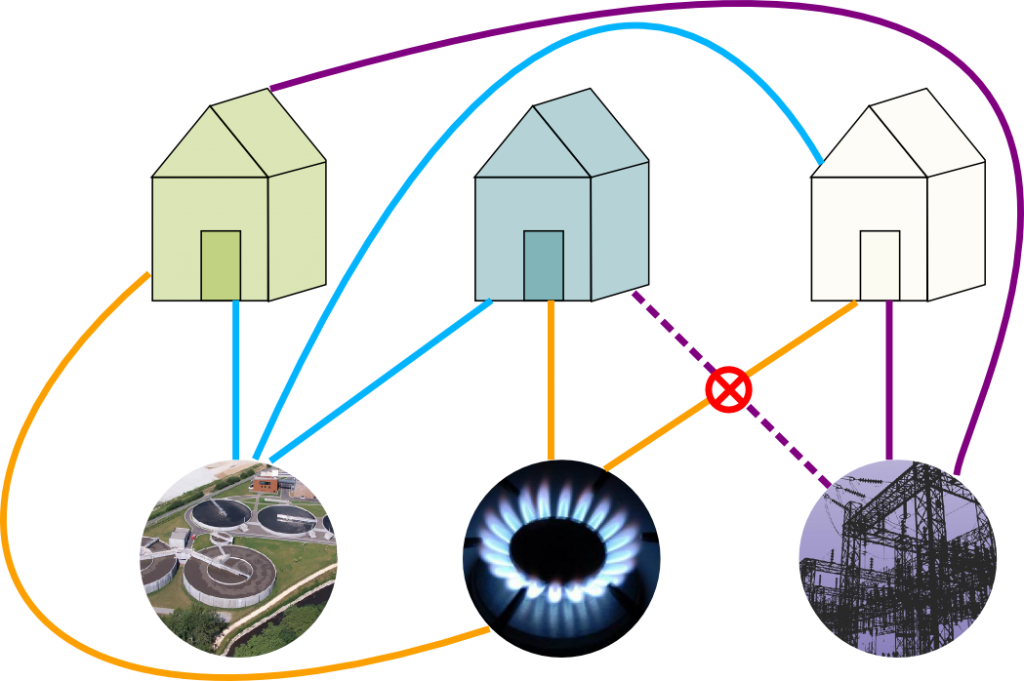
\includegraphics{The-Utilities-Problem-Bad-Solution.png}
\caption{Attempt at solving the three utilities problem}
\end{figure}

However, this just shows one attempt at connecting them up fails; it
seems very hard to prove that no such attempt could succeed, as there
are lots of ways you could try to draw it. However, later in this
lecture we will show that it is impossible. But first

\subsubsection{A notational interlude:}\label{a-notational-interlude}

In the graph we are trying to draw in the Three Utilities Problem, we
have two different types of vertices: the houses, and the utility
factories. The graph only has edges between vertices of one type and
vertices of the other type. Similar graphs occur frequently, and so we
make the following definition:

We have typically viewed graphs as drawings in the plane, with the
vertices as dots and the edges as lines between them. Different choices
of drawings of them same graph can look very different (as we saw with
the Petersen graph). One thing that is convenient is to have drawings
where the edges never cross (we might wonder if the crossing is a
vertex). We are naturally then led to the following definition:

\subsection{Definition}\label{definition-10}

A graph is \emph{planar} if it can be drawn in the plane
(\(\mathbb{R}^2\)) so that none of the edges cross.

\subsection{Definition}\label{definition-11}

A graph is \emph{bipartite} if its vertices can \(V(\Gamma)\) and can be
separated into two sets, \(U\) and \(W\), so that any edge of goes
between a vertex of \(U\) and a vertex of \(W\).

The very first picture on the
\href{https://en.wikipedia.org/wiki/Bipartite_graph}{wikipedia entry} is
the picture you should have in your head.

\subsection{Example}\label{example-7}

The 4 cycle \(C_4\) is bipartite, while the 3 or 5 cycles are not.

A special case is when every vertex of \(U\) and is connected to every
vertex of \(W\) -- i.e., the graph has many edges as it can while still
being simple and bipartite.

\subsection{Definition}\label{definition-12}

The complete bipartite graph \(K_{m,n}\) has \(m+n\) vertices, split
into a set \(U\) with \(m\) vertices and \(W\) with \(n\) vertices. For
every \(u\in U\) and \(w\in W, K_{m,n}\) has exactly one edge.

\subsection{Back to the puzzle:}\label{back-to-the-puzzle}

Returning back to the Utilities Problem, it should be fairly clear that
it is equivalent to the following question: Is \(K_{3,3}\) is planar?
Our next goal is to prove that it is not.

\subsubsection{A tiny bit of topology}\label{a-tiny-bit-of-topology}

Since we're trying to draw it in the plane, we are secretly starting to
do a little bit of topology. This is not a module on topology, and we
will do as little as we can get away with, but it may help to highlight
slightly where we use a little. In particular, the main idea of the
proof will use some form of the
\href{https://en.wikipedia.org/wiki/Jordan_curve_theorem}{Jordan Curve
Theorem}, which basically says that if we draw a simple closed curve
(i.e., a circle) in the plane, it cuts it into two pieces, an inside and
an outside. This certainly sounds intuitively obvious, and would go
without question to anyone besides a mathematician -- think about some
of the nasty curves you encountered in Analysis!

\subsection{Main idea of the proof}\label{main-idea-of-the-proof}

The problem with trying to show a graph is nonplanar is that it seems at
first glance that there are tons of possible ways to try to draw it in
the plane, and so the proof would have a huge number of different cases,
and it would be tricky to make sure you'd covered them all. The main
idea of the proof is to use the Jordan curve theorem as a way to
eliminate a lot of cases and organize the remaining ones. This idea is
widely applicable, and in previous versions of the course was referred
to as the ``planarity algorithm'', although we will not formalise it to
the level of an algorithm.

The idea is the following: suppose that a graph \(\Gamma\) was planar,
and consider some closed walk \(W\) in \(\Gamma\) that doesn't repeat
any vertices. Then if we draw \(\Gamma\) in the plane, then \(W\) will
be a circle, and so by the Jordan curve theorem every vertex or edge not
in \(W\) must either be on the inside or outisde of \(W\). One can then
do a case-by-case analysis placing each vertex or edge inside or
outside.

Obviously, the fewer vertices and edges that aren't contained in \(W\),
the fewer cases our proof will have, and so in the best case )and the
only ones we will consider) we take \(W\) to be a Hamiltonian cycle.

\subsection{\texorpdfstring{Proof that \(K_{3,3}\) isn't
Planar}{Proof that K\_\{3,3\} isn't Planar}}\label{proof-that-kux5f33-isnt-planar}

Let the vertices \(a,b,c\) be coloured red and vertices \(x,y,z\) be
coloured blue. The path \(a-x-b-y-c-z-a\) is a Hamiltonian cycle, that
we draw as a circle in the plane, as shown below:

This contains 6 of the 9 edges of \(K_{3,3}\); we need to add the edges
\(a-y, b-z\) and \(c-x\). The edge \(a-y\) could be drawn inside the
circle or outside, suppose we draw it inside, as shown below, with the
added edge dashed.

Then on the inside of the circle, \(x\) and \(c\) are on different sides
of the line \(a-y\), and so the edge connecting them must go outside the
circle. The added edge could go around the right of the circle, as shown
below here:

or around the left, as shown here:

But now \(b\) and \(z\) are different sides of \(a-y\) inside the
circle, and on different sides of \(c-x\) outside the circle, and so
cannot be connected without making two edges cross.

If we had began by drawing \(a-y\) outside the circle, then we would
have had to draw \(c-x\) inside the circle, and had the same problem
with being able to draw the last line; as shown here:

\subsection{An unnecessary case and steoreographic
projection}\label{an-unnecessary-case-and-steoreographic-projection}

In the proof as presented, we do two cases that seem essentially
identical -- namely, whether the first edge \(a-y\) was drawn inside the
circle or outside the circle. In a good proof you don't want to consider
more cases than necessary, so it's worth stopping to see if these cases
are really ``the same'' or not.

At first glance, the inside and outside of the circle seem to appear
very different: the inside has finite area, while the outside has
infinite area. However, here's a slightly different situation where the
inside and outside are obviously interchangable: replace \(\R^2\) with
the sphere \(S^2\), and draw the circle as the equator. Then the
``inside'' is the northern hemisphere, and the ``outside'' is the
southern hemisphere, and obviously we can just do a reflection to
interchange them.

It seems like a huge leap to replace the plane with the sphere, but the
sphere is really just the plane with one additional point! Put another
way, suppose we could draw \(\Gamma\) on the sphere. Our drawing would
miss at least point, and if we cut open the sphere at that one point we
could stretch the sphere out and lay it flat on the plane, giving a
drawing of \(\Gamma\) on the plane.

That sounded vague, but one way it can be made precise is the following:
through
\href{https://en.wikipedia.org/wiki/Stereographic_projection}{stereographic
projection}, which the wikipedia page makes look complicated, but is
really just this picture:

\begin{figure}[htbp]
\centering
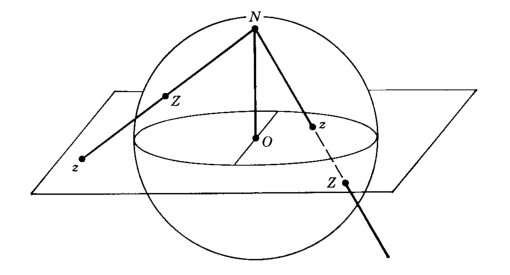
\includegraphics{stereographicprojection.jpg}
\caption{Stolen stereographic projection picture}
\end{figure}

Draw the sphere as the unit sphere centerred at the origin, so the North
pole is the point \(N=(0,0,1)\). Then, for any point \(Z\neq N\) on the
sphere, there is a unique line through \(N\) and \(Z\). That line will
meet the \(xy\) plane in a unique point \(z\). Similarly, given any
point \(z\) in the \(xy\) plane, the line through \(z\) and \(N\) will
meet the sphere in one other point \(Z\). This gives a bijection between
points on the plane, and points on there sphere (except for the north
pole).

If discussion above we slightly lacking, there are lots of
\href{https://www.youtube.com/watch?v=6JgGKViQzbc}{fun videos} showing
(variations of) stereographic projection on youtube. I mentioned in
particular \href{https://www.youtube.com/watch?v=VX-0Laeczgk}{Henry
Segerman's videos} that illustrated this using shadows and 3-d printed
spheres.

\subsubsection{Back to planar graphs}\label{back-to-planar-graphs}

If that digression into topology seemed long and pointless, the upshot
is that if we're trying to prove a Hamiltonian graph is nonplanar, we
can treat the inside and the outside of the circle as equivalent, and so
when we try to add the very first edge we may as well put it inside.
This gives us one less choice, and so makes our proofs about half as
long! We will use this trick to show that:

\subsection{\texorpdfstring{The complete graph \(K_5\) isn't
planar}{The complete graph K\_5 isn't planar}}\label{the-complete-graph-kux5f5-isnt-planar}

The proof is similar, in that we begin by picking a Hamiltonian cycle,
say, \(a-b-c-d-e-a\), and drawing this as a cirlce in the plane, and
then try to add the remaining edges. \(K_5\) has \(5\cdot 4/2=10\)
edges, and 5 are contained in the cycle, so we have 5 more edges to add
-- \(a-c, a-d, b-d,b-e\) and \(c-e\).

Since the inside and outside of the circle are equivalent, we will
assume the first edge \(a-c\) is drawn \emph{inside} the circle, giving
us the following picture:

It may be tempting to next consider the edge \(a-d\), but this could be
drawn either inside or outside the circle, and so we'd have to start
considering cases. We get a shorter, cleaner proof if we now move on to
the vertex \(b\).

The vertex \(b\) is separated from \(d\) and \(e\) on the inside of the
circle by the line \(ac\), and hence the edges \(b-e\) and \(b-d\) must
be drawn on the outside of the circle. These edges separate \(a\) from
\(d\) on the outside of the circle, and so this must be drawn inside,
giving the following picture:

But now we cannot add the final \(c-e\), as \(c\) and \(e\) are
separated from each other on both the outside and the inside of the
circle.

\(\square\)

\section{Lecture 14: Kuratowski's theorem; graphs on the torus and Mobius band}

Last session we proved that the graphs \(K_{3,3}\) and \(K_5\) are not
planar. We now discuss Kuratowski's theorem, which states that, in a
well defined sense, having a \(K_{3,3}\) or a \(K_5\) are the
\emph{only} obstruction to being non-planar.

We begin with some two simple observations.

\subsection{Observation 1}\label{observation-1}

If \(H\) is a subgraph of \(G\), and \(H\) is not planar, then \(G\) is
not planar.

\subsection{Proof}\label{proof-11}

If we could draw \(G\) in the plane, it would produce a drawing of \(H\)
in the plane, a contradiction. \(\square\)

As an immediate corrolary, we see that \(K_n\) is not planar for
\(n\geq 5\), as all such complete graphs contain \(K_5\) as a subgraph;
similarly, \(K_{m,n}\) are not planar, with \(m,n\geq 3\).

Our second observation is the following: suppose we took a graph
\(\Gamma\), and made a new graph \(\Gamma^\prime\) by adding one vertex
of degree 2 in the middle of one of the edges of \(\Gamma\). Then
drawing \(\Gamma^\prime\) is basically the same as drawing \(\Gamma\),
and then sticking an extra dot on an edge. Hence, \(\Gamma^\prime\) will
be planar if and only if \(\Gamma\) was.

We now make this precise:

\subsection{Definition}\label{definition-13}

We say that \(\Gamma^\prime\) is a subdivision of \(\Gamma\) if it is
obtained from \(\Gamma\) by repeatedly choosing an edge \(e\) and
splitting it into two by adding a new vertex, as in the following
picture:

\begin{figure}[htbp]
\centering
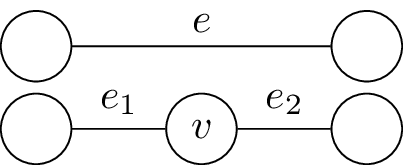
\includegraphics{../TeXpictures/split.png}
\caption{Splitting/Joining an edge}
\end{figure}

\subsection{Observation 2}\label{observation-2}

Suppose that \(\Gamma^\prime\) is a subdivision of \(\Gamma\). Then
\(\Gamma^\prime\) is planar if and only if \(\Gamma\) is.

\subsection{Example}\label{example-8}

The following graph \(G\) is nonplanar, since it is obtained from
\(K_{3,3}\) by subdividing a single edge.

\begin{figure}[htbp]
\centering
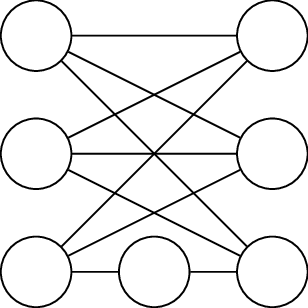
\includegraphics{../TeXpictures/K33homeo.png}
\caption{K33 Subdivision}
\end{figure}

Putting together the two lemmas, we see that if \(G\) has a subgraph
\(H\), so that \(H\) is a subdivision of a non-planar graph (like
\(K_5\) or \(K_{3,3}\)), then we \(G\) isn't planar. We illustrate this
now in an exmaple.

\subsection{Example: The Petersen graph is not
planar}\label{example-the-petersen-graph-is-not-planar}

\begin{figure}[htbp]
\centering
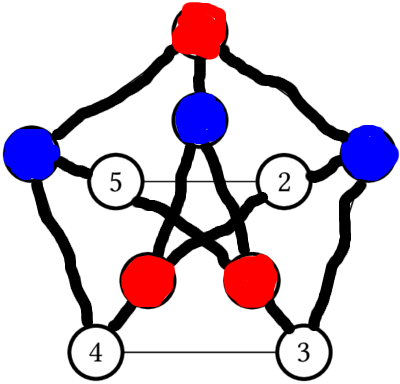
\includegraphics{../TeXpictures/PetersenNonPlanar.png}
\caption{PetersenSubgraph}
\end{figure}

The subgraph drawn with thick edges (containing all but two of the edges
in the Petersen graph) is homeorphic to \(K_{3,3}\). we have drawn three
vertices blue and three vertices red to highlight the vertices of
\(K_{3,3}\). The nonhighlighted edges are in the subgraph, but they are
the ones that are forgetten to show that the highlighted graph is
homeomorphic to \(K_{3,3}\).

\subsection{Kuratowski's Theorem}\label{kuratowskis-theorem}

A graph \(G\) is nonplanar if and only if it contains a subgraph
homeomorphic to \(K_5\) or \(K_{3,3}\).

Our two observations, together with this morning's result that
\(K_{3,3}\) and \(K_5\) are nonplanar, prove the ``if'' direction. The
``only if'' direction is much harder, and we will not prove it.

However, we will only use the ``only if'' direction implicitly. Using
the ``only if'' direction explicitly would amount to prove that some
graph was planar by showing it had no subgraphs that were subdivisions
of \(K_5\) or \(K_{3,3}\), which we would be quite laborious. We have a
much easier way to prove that a graph \emph{is} planar: drawing it in
the plane.

We will however, use the ``only if'' direction implicitly in the
following way. Suppose we have a graph \(G\), and we want to determine
if \(G\) is planar or not. We can try to prove it is planar by trying to
draw it in the plane, and we can try to prove it is not planar by
finding a subgraph of \(G\) that is homeomorphic to either \(K_{3,3}\)
or \(K_5\). The ``only if'' direction of Kuratowski's theorem tells us
that one or the other of these attempts will \emph{always} work. Thus,
we have a practical method to determine whether or not a graph is planar
or not -- try to draw it in the plane. If you find this difficult, and
begin to expect that it isn't possible, start looking for a subgraph
homeomorphic to either \(K_5\) or \(K_{3,3}\), which would prove it
can't be drawn on the plane.

\subsubsection{Graphs on other surfaces}\label{graphs-on-other-surfaces}

We now transition to drawing graphs on other surfaces. In lecture, we
had some slides providing pictures for the beginning of this discussion;
a few, but not all, of those images are in the body of these notes now.

Trying to draw graphs on surfaces can be fun, but it seems like a rather
unmotivated question to consider, so we began with motivating it by
videogames. Many videogames (pacman, asteroids, overhead RPGs like the
early Final Fantasy games) take place on a rectangle screen:

\begin{figure}[htbp]
\centering
\includegraphics{../Slides/Pictures/chronostatic.gif}
\caption{Videogame map}
\end{figure}

To avoid making the world have an ``edge'', the result will often
happen: if a character moves off the right of the screen it will
reappear at the edge of the left screen, and similarly if a character
moves off the top of the screen, it reappears on the corresponding place
on the bottom of the screen.

This set-up is used to simulate the surface of a planet. However, if one
traces through the result of these identifications, one sees that the
surface is a torus:

\begin{figure}[htbp]
\centering
\includegraphics{../Slides/Pictures/chronofolding.gif}
\caption{map folding}
\end{figure}

\subsection{Definition}\label{definition-14}

A ``video-game graph'' is one that ``locally looks like'' a part of
graph paper.

\subsection{Motivating Question}\label{motivating-question}

If videogame designers were more clever, could they put a finite
videogame graph on the sphere? Can you prove that it isn't possible?

\subsubsection{Drawing graphs on the
torus}\label{drawing-graphs-on-the-torus}

If we wanted to draw a graph on the sphere, we could do this physically
by taking a balloon and a felt pen, but it would be a little awkward to
turn in or mark homeworks this way. Luckily, we saw last time that,
using stereographic projection, drawing a graph on the sphere is
equivalent to being able to draw it on the plane.

Similarly, we could draw graphs on torus by getting donuts, and writing
on them with icing sugar. But again, this is rather impractical, and
we'd like a way to represent drawing a graph on a torus that is
conveniently done on a piece of paper.

The videogame / paper-folding discussion shows us how to do this. We
draw a square to represent the torus. On the top and bottom border we
draw one arrow in the same direction, to signify that these edges will
be identified (this is how the paper was folded, or what a character
does in the videogame). We do similar with the side borders, with two
arrows.

Then we can draw the graph in the square, with the following added
options -- if a drawn edge reaches the left (right) border, it continues
at the same spot on the right (left) border, and similarly with the
top/bottom borders.

\subsection{Example}\label{example-9}

\(K_5\) and \(K_6\) cannot be drawn on the plane, but they can be drawn
on the torus as follows:

\begin{figure}[htbp]
\centering
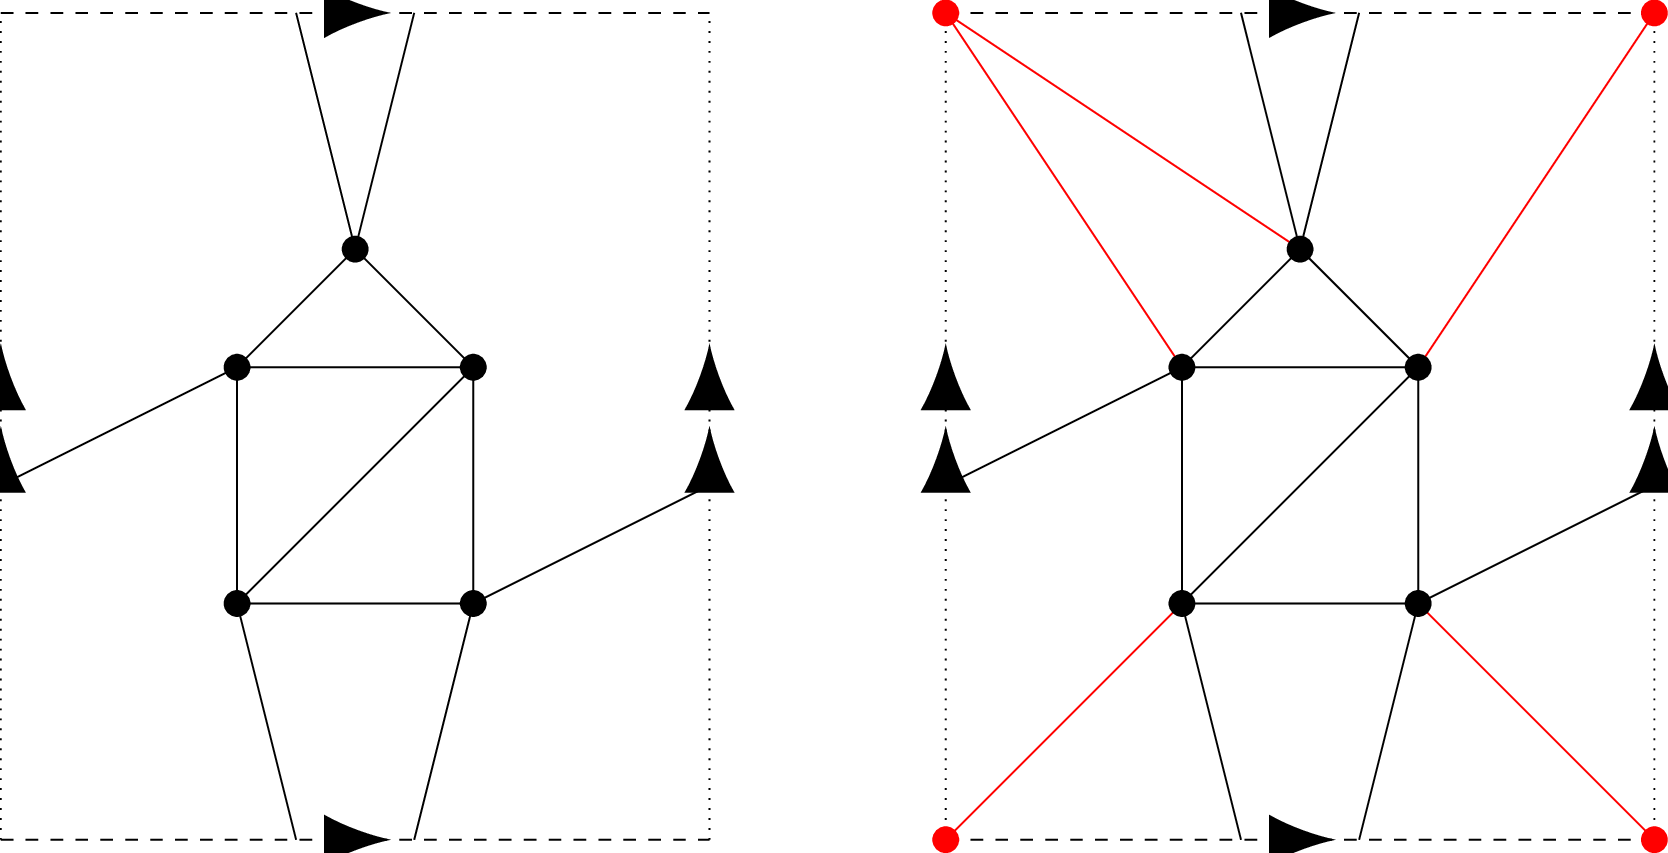
\includegraphics{../TeXpictures/K5K6torus.png}
\caption{K5 and K6 on the torus}
\end{figure}

The graph on the left shows \(K_5\) on the torus. The picture on the
right has the same drawing of \(K_5\) in black, but in red has added an
extra vertex and 5 extra edges incident to it to make a \(K_6\). There
are appear to be 4 red vertices, at each corner of the square, but since
all the corners get identified by the folding, they correspond to the
same point of the torus.

\subsection{Challenge}\label{challenge}

Draw \(K_7\) on the torus.

It turns out that \(K_8\) cannot be drawn on the torus -- we will not quite be able to prove this, but it follows from something very similar to Euler's theorem.



\subsubsection{What comes next?}\label{what-comes-next}

What other surfaces other than the sphere and torus are possible? One
possibility is just adding ``more holes''; this produces the ``donut
with \(g\) holes'', more formally known as the ``suface of genus
\(g\)''.

You won't have to work with surfaces of higher genus, but it is worth
knowing that this is an active area of research and investigation. It
turns out (try to prove it! It's not hard\ldots{}) that given any finite
graph \(\Gamma\), there is some \(g\) so that \(\Gamma\) can be drawn on
a surface of genus \(g\) without the edges crossing. The \emph{genus} of
a graph \(\Gamma\) is defined to be the lowest \(G\) such that this can
be done.




\subsection{Nonorientable Surfaces}\label{nonorientable-surfaces}

Although you won't have to work with surfaces of higher genus, you will
have to be able to work with a couple of other surfaces. We will end
this lecture by introducing the Mobius band:

\subsubsection{Unorientable surfaces}\label{unorientable-surfaces}

In this half of the lecture, we introduce the real projective plane, the
simplest closed compact unorientable surface.

Before we do that, it is easiest to review an unorientable surface with
boundary that may be more familiar: the Mobius band.

\subsection{The Mobius band}\label{the-mobius-band}

Suppose one has a strip of paper and glues the opposite edges together
in the natural way -- this makes a cylinder.

If instead, one glued the ends together with half a twist, one would get
the Mobius band:

\begin{figure}[htbp]
\centering
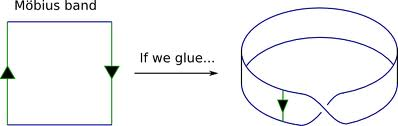
\includegraphics{../Slides/Pictures/mobiusglue.jpg}
\caption{mobius band glue}
\end{figure}

The mobius band is not the same topological space as the cylinder. One
way to see this is that it is \emph{unorientable} -- there is not a
consistent notion of left and right on the Mobius band. If you start at
one point on the Mobius band, and travel along it until you jump across
the other side of the identification, you will eventually return to
where you started. However, your left and right will have been
interchanged! This is seen in the following pictures,
\href{https://haggisthesheep.wordpress.com/2009/06/15/mobius-strips/}{stolen
from this blog post}:

\begin{figure}[htbp]
\centering
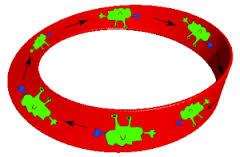
\includegraphics{../Slides/Pictures/mobiusunorientable.jpg}
\caption{courtesy haggisthesheep.blogspot.com}
\end{figure}

The creature started out, his right hand was blue, but when he returns
from his trip around the mobius band it is now his left hand that is
blue!

\section{Lecture 15: Unorientable surfaces, classification of surfaces, dual graphs}

\subsubsection{More Mobius}\label{more-mobius}

At the end of the last lecture we briefly introduced the Mobius band.
This lecture, we briefly recalled what the Mobius band looked like,
noted that it only has one edge, and as a warm-up drew \(K_{3,3}\) on
the Mobius band.

We noted that the Mobius band only had one edge; which didn't seem so
scary. However, this means that if you cut the Mobius band down the
middle, it doesn't split into two pieces! Note that this violates the
Jordan curve theorem, the intuitive seeming that every circle as an
inside and an outside.

\subsection{Real Projective Plane}\label{real-projective-plane}

The Mobius band is nice, but it's a little annoying that it's just a
surface with boundary, not just a surface -- you could walk off the
edge. However, we can fix this, by taking a disk, and gluing it to the
Mobius band along the boundary circles. The result is called the (real)
projective plane, and written \(\mathbb{RP}^2\). The projective plane is
a closed, compact surface, but you can't draw it in \(\mathbb{R}^3\)
without it passing through itself.

We need a planar representation of the projective plane, along the same
lines as our planar representations of the surface of genus \(g\) we
gave in the first half of this lecture. To do this, we claim that the
real projective plane is the same as the disk with opposite sides of the
boundary identified, as in the following picture:

\begin{figure}[htbp]
\centering
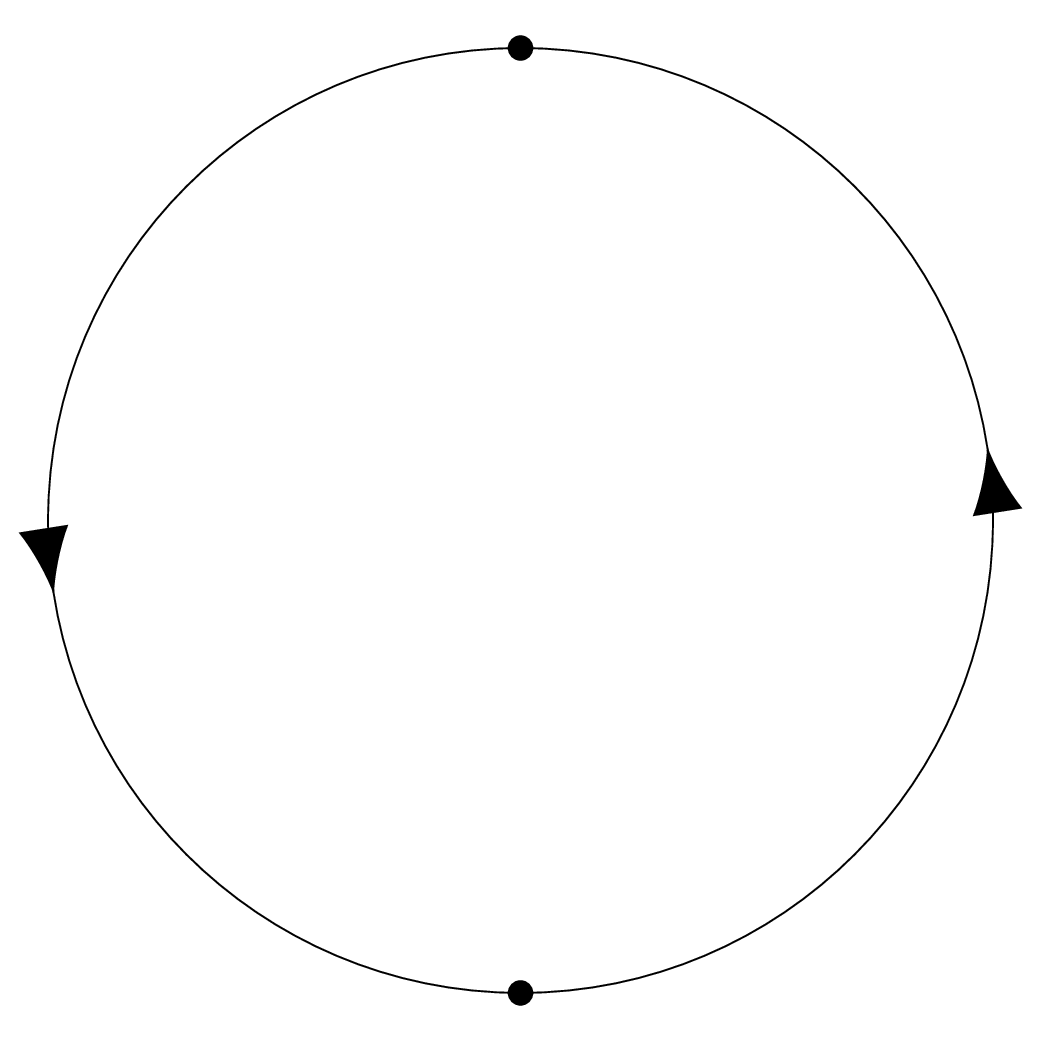
\includegraphics{../LatexPictures/RP2.png}
\caption{RP2 is the disk with opposite points on the boundary
identified}
\end{figure}

We now have two descriptions of \(\mathbb{RP}^2\) -- as a mobius band
glued to a disk, and as a disk with opposite points on the boundary
identified. We should check that they are the same, which can be done by
cutting and pasting, as illustrated in the following picture:

\begin{figure}[htbp]
\centering
\includegraphics{../Slides/Pictures/MobiusRP2.gif}
\caption{Equivalence between the two descriptions of RP\^{}2}
\end{figure}

The part labeled {[}1{]} begins with a disk with opposite parts of the
boundary identified. We cut a strip \(J\) out of the middle of the disk
-- this is the Mobius band.

The remaining pieces \(F\) and \(R\), when we glue them together as the
boundary of the disk was, becomes just a disk.

The part labelled {[}2{]} is another way to see it that is the inverse
of what I drew on the board.

Just as we argued that a graph was planar if and only if it could be
drawn on the sphere, one can show:

\subsection{Lemma}\label{lemma-7}

A graph \(\Gamma\) can be drawn on \(\mathbb{RP}^2\) if and only if
\(\Gamma\) can be drawn on the Mobius band.

\subsection{Proof}\label{proof-12}

Since we obtain \(\mathbb{RP}^2\) by adding things, clearly if we can
draw \(\Gamma\) on the Mobius band we can draw it on the projective
plane.

To go the other direction, not that any drawing of \(\Gamma\) will leave
some white space, and we can just cut a small disk out of the missed
area to get a Mobius band.

\subsection{\texorpdfstring{Graphs on
\(\mathbb{RP}^2\)}{Graphs on \textbackslash{}mathbb\{RP\}\^{}2}}\label{graphs-on-mathbbrp2}

Since we have a planar representation of \(\mathbb{RP}^2\) we have a
handy way to draw graphs on it. We draw a graph inside a circle, and if
we can draw edges that hit the boundary of the circle, and they will
continue on the other side.

As an example, we show how \(K_5\) can be drawn on \(\mathbb{RP}^2\)
below:

\begin{figure}[htbp]
\centering
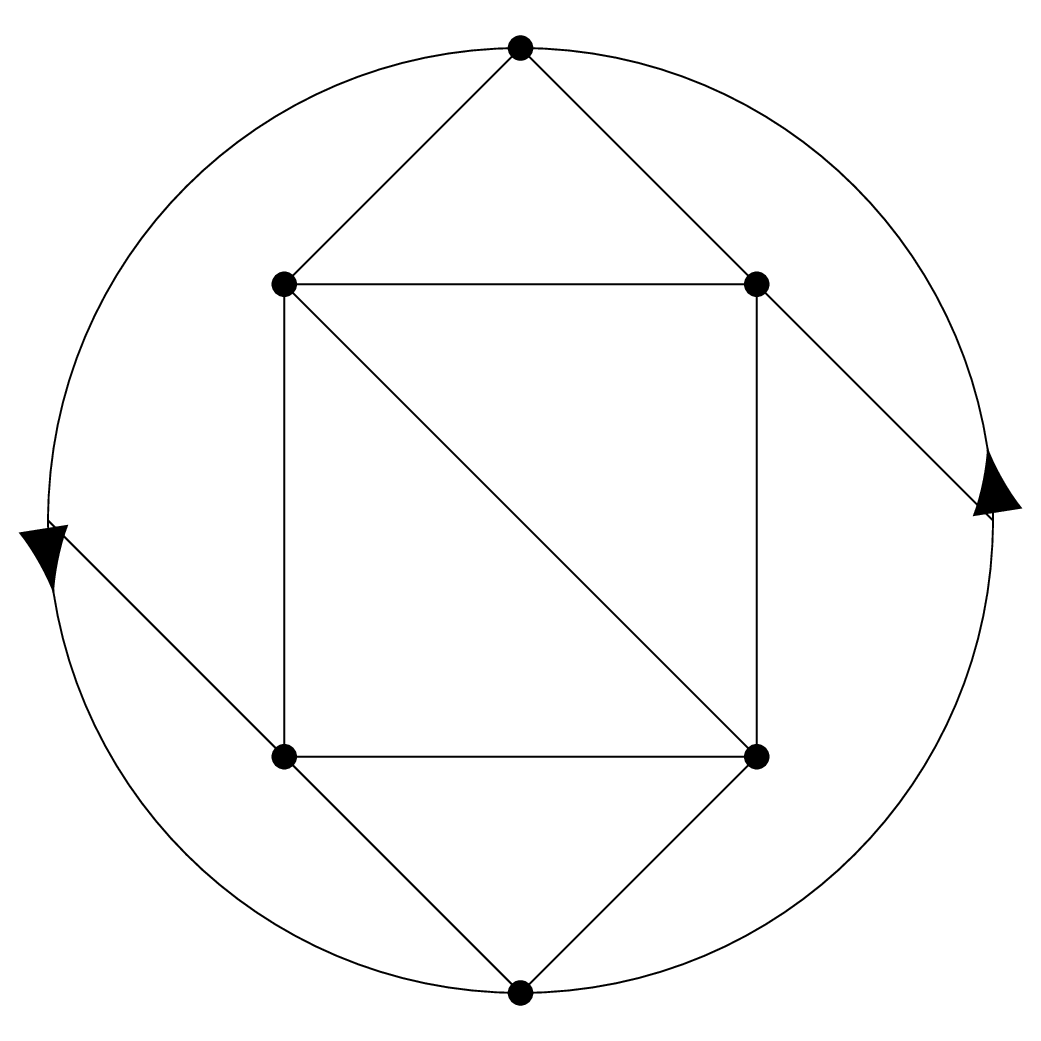
\includegraphics{../LatexPictures/rp2k5.png}
\caption{K5 drawn on RP2}
\end{figure}

Four of the vertices are in the interior of the circle, the fifth vertex
is on the boundary and hence appears twice, at the very top and very
bottom. The edge from the upper right vertex going diagonal down hits
the boundary at the very right, and then continues on its way starting
again from the very left.

\subsection{Klein Bottle}\label{klein-bottle}

When we glued a disk to the boundary of the Mobius band, we could
instead of glued the boundary of a second Mobius band to them. This
\href{https://www.youtube.com/watch?v=a5Azcwe9p4o}{this youtube video}
illustrates that process, but it is probably easier to do a cut and
paste computation similar to how we constructed our presentation of the
projective plane, we see that the surface this results in looks a lot
like the Torus, but with one of the sets of identifications done
backwards:

\begin{figure}[htbp]
\centering
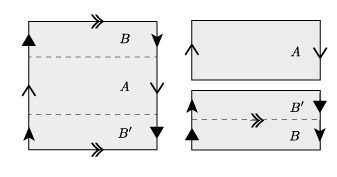
\includegraphics{kleinto2moebius.png}
\caption{Klein bottle is two Mobius bands}
\end{figure}

The resulting surface is called the \emph{Klein bottle}; again, the
Klein Bottle is unorientable and cannot be drawn in \(\R^3\) without
crossing over itself; it is usually drawn in \(\R^3\) as follows:

It is most conveniently pictured as a square with the opposite sides
identified, but with one pair of sides reversed, as seen in the
following picture.

\begin{figure}[htbp]
\centering
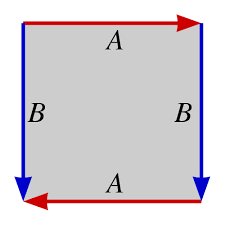
\includegraphics{../Slides/Pictures/KleinSquare.png}
\caption{Klein Bottle is a square with sides identified}
\end{figure}

It is not too hard to visualize that this identification pattern gives
the picture above. If we identify the blue edges marked \(B\) we just
get the cylinder. Now, we have to identify the ends of the cylinder, but
with the orientations reversed; to do this we have to pass through the
surface itself as seen in the picture.

\subsubsection{Mathematical Cultural Literacy: The classification of
surfaces}\label{mathematical-cultural-literacy-the-classification-of-surfaces}

You will only be responsible for being able to draw graphs on the four
simplest surfaces: The sphere, the torus, the projective plane, and the
Klein bottle. However, it is natural to ask what other surfaces are
possible, and how to represent them in the plane.

It turns out that if you take any polygon with an even number of sides,
and randomly glue them together in pairs in some order and choice of
orientation, you will get a closed compact surface, and every closed
compact surface can be gotten in this way (but not uniquely).

The following picture shows how this is done with surfaces of genus 1, 2
and 3.

\begin{figure}[htbp]
\centering
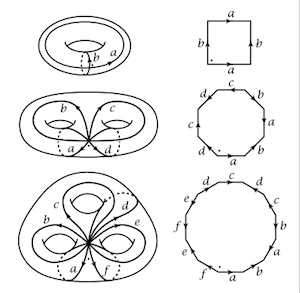
\includegraphics{../Slides/Pictures/genus123.png}
\caption{Low genus surfaces}
\end{figure}

It can be hard to visualize how folding the \(4g\)-gon up produces a
genus \(g\) surface; This video shows this in the case of a two-holed
surface that should make it clear.

\subsection{Classification of Surfaces}\label{classification-of-surfaces}

Every closed compact surface is either 1. The surface of genus \(g\),
for \(g\geq 0\) 2. The sphere with \(k>0\) circles cut out, and a Mobius
band

The surfaces in Option 1 are the orientable surfaces, the surfaces in 2.
are the unorientable surfaces.

\subsubsection{Dual graphs}\label{dual-graphs}

In the examples at the very beginning of the course, we got a graph from
a drawing on the sphere: the Risk board, or more generally, any map.

The countries (or counties or states or whatever region we are working
with) are the vertices, and two countries are adjacent if they share a
border.

This is different from how we have been thinking about drawing graphs on
surfaces -- for us, the places where more than two countries meet would
be the vertices, and the borders would again be edges. But both of these
graphs are coming from the same drawing on the sphere, and so must be
related somehow; the concept of \emph{dual graphs} makes this precise.

\subsection{Definition}\label{definition-15}

Let \(\Gamma\) be drawn on a surface \(S\). The connected components of
\(S\setminus\Gamma\) -- i.e., the pieces we would have if we cut \(S\)
along \(\Gamma\) -- are called \emph{faces}

Note: by the Jordan curve theorem, on a sphere, each face will just be a
disk. However, this need not be true on a regular surface -- for
instance, we can get a cylinder as a connected region on the Torus, and
the Mobius band as a connected region on the projective plane.

\subsection{Definition}\label{definition-16}

Let \(\Gamma\) be drawn on a surface \(S\), with vertices \(v\). The
\emph{dual graph} of \(\Gamma, S\) is the graph with a vertex for each
face of \(\Gamma, S\), and an edge for each edge of \(e\in E(\Gamma)\),
that connects the two faces that \(e\) separates.

\subsubsection{\texorpdfstring{It is not hard to see that the faces of the
dual graph are the vertices of the original graph, and hence that the
dual of the dual graph of \(\Gamma\) is the original graph \(\Gamma\)
back.}{It is not hard to see that the faces of the dual graph are the vertices of the original graph, and hence that the dual of the dual graph of \textbackslash{}Gamma is the original graph \textbackslash{}Gamma back.}}\label{it-is-not-hard-to-see-that-the-faces-of-the-dual-graph-are-the-vertices-of-the-original-graph-and-hence-that-the-dual-of-the-dual-graph-of-gamma-is-the-original-graph-gamma-back.}

\section{Lecture 16: Euler's Theorem and applications}

We ended this morning's lecture by introducing the concept of the face
of a graph, and of the dual graph. In this lecture we prove Euler's
theorem, which gives a relation between the number of edges, vertices
and faces of a graph.

We begin by counting the number of vertices, edges, and faces of some
graphs on surfaces -- the tetrahedron (or triangular pyramid) has 4
vertices, 6 edges, and 4 faces; the cube has 6 vertices, 12 edges, and 8
faces, etc.

\subsection{Euler's Theorem}\label{eulers-theorem}

Let \(\Gamma\) be a graph drawn on the sphere, and suppose that
\(\Gamma\) has \(v\) vertices, \(e\) edges, and \(f\) faces. Then
\(v-e+f=2\).

\subsection{Proof idea 1:}\label{proof-idea-1}

One way to prove it is the following: if we delete an edge from
\(\Gamma\), we will (usually) merge two faces into one, and thus have
one less edge and one less face; this does not change \(v-e+f\).

Similarly, if we have a vertex of degree 2, we can delete it and merge
the two edges into one, getting one less edge and one less vertex, which
does not change \(v-e+f\).

By iteratively doing this two moves, you can get to a very basic graph
or two, which you can check have \(v-e+f=2.  \square\)

\subsection{Proof 2: Dual spanning
trees}\label{proof-2-dual-spanning-trees}

First, take a spanning tree \(T\) of \(\Gamma\); it has \(v\) vertices,
and since it is a tree it must have \(v-1\) edges.

Now, we construct another graph \(\tau\) as follows. The vertices of
\(\tau\) will be the faces of our original graph \(\Gamma\). We will
connect two vertices of \(\tau\) if and only if they are connected by an
edge \emph{not} in our spanning tree \(T\). Thus, we see that \(\tau\)
is a subgraph of the dual graph of \(\Gamma\), that contains all the
vertices and every edge that isn't in \(T\).

We first note that Euler's formula follows if we can show that \(\tau\)
is a tree as well, as then \(\tau\) would have \(f\) vertices and hence
\(f-1\) edges. But since every edge of \(\Gamma\) is either in \(T\) or
\(\tau\) we have

\[v-e+f=|V(T)|-|E(T)|-|E(\tau)|+|V(\tau)|=1+1=2\]

To prove that \(\tau\) is indeed a tree, we need to show \(\tau\) is
connected and has no cycles. If \(\tau\) were disconnected, then we
claim \(T\) would have a cycle. Let \(\tau_1\subset \tau\) be one of the
connected components, and consider the union of all the faces in
\(\tau_1\). This is some region of the sphere that isn't the whole
thing; its boundary will be a union of circles. But the boundary is also
a union of edges in \(T\); therefore, \(T\) must contain a cycle, a
contradiction.

We also need to show that \(\tau\) has no cycles; this is just the
``dual'' of the above argument: But if \(\tau\) had a cycle, it would
cut the sphere into two pieces, each of which would contain a vertex of
\(T\), and hence \(T\) would be disconnected, a contradiction.
\(\square\)

\subsubsection{Applications of Euler
characteristic}\label{applications-of-euler-characteristic}

Euler's theorem can be very useful in proving results about graphs on
the sphere. It's a bit awkward to use by itself -- it contains three
variables, \(v, e\) and \(f\), so it is most useful when we already know
some relations between these variables. This may be best illustrated by
our motivating example:

\subsection{Theorem}\label{theorem-1}

It is impossible to draw a sphere with a videogame graph.

\end{document}

\begin{document}
\subsection{Proof}\label{proof-13}

Recall that in a videogame graph, every vertex had degree 4, and each
face was a square.

Suppose that we had such a graph drawn on the sphere; Euler's theorem
gives us \(v-e+f=2\); we need to use our other knowledge about the graph
to get a contradiction.

How can we use that every vertex has degree 4? The handshaking lemma!
Since every vertex has degree 4, the sum of the degrees of the vertices
is just \(4v\). So the Handshaking Lemma just says \(4v=2e\), and hence
\(e=2v\).

How can we use that every face has four sides? We can do something just
like the handshaking lemma, and count the number of times a face meets
an edge. On the one hand, each edge meets two faces, and so there are
\(2e\) places that an edge meets a face. On the other hand, each face
meets four edges, and so we see there are \(4f\) times a face meets an
edge, and so we have that \(2e=4f\), or \(e=2f\).

Putting \(e=2v\) and \(e=2f\) together, we see that \(f=v\), and so
\(v-e+f=v-2v+v=0\), which is a direct contradiction of Euler's Formula
\(,\quad \square\)

It's worth noting that ``handshaking between edges and faces'' actually
\emph{is} the handshaking lemma for the dual graph.

To generalize this, we note that we have three sources of relationships
between \(v, e\) and \(f\) for a planar graph:

\begin{enumerate}
\def\labelenumi{\arabic{enumi}.}
\tightlist
\item
  Euler's Formula
\item
  Handshaking between vertices and edges
\item
  Handshaking between edges and faces
\end{enumerate}

These three relations can work together to prove a lot. We give one more
example now -- another proof that \(K_5\) and \(K_{3,3}\) aren't planar.
Yet another example can be found on the last homework set -- figuring
out how many pentagons a football has.

\subsection{\texorpdfstring{Application: \(K_5\) and \(K_{3,3}\) aren't
planar}{Application: K\_5 and K\_\{3,3\} aren't planar}}\label{application-kux5f5-and-kux5f33-arent-planar}

Let's try to give another proof that \(K_5\) and \(K_{3,3}\) aren't
planar using Euler's formula.

First, let's show \(K_5\) isn't planar. We know explicitly that \(K_5\)
has 5 vertices and 10 edges, so if it were drawn on the sphere we would
have

\[2=v-e+f=5-10+f=f-5\]

and so it would have to have 7 faces. To get a contradiction, we need
another way to get information about how many faces the drawing would
have, which we can do via handshaking. \(K_5\) has no multiple edges or
loops, and so the smallest number of edges a face could have is 3. Thus,
handshaking gives us

\(2e=\sum_{f \text{ face} } d(f)\geq \sum_f 3=3f\) i.e., \(2e\geq 3f\).
But we know \(e=10\) and \(f=7\), so we have a contradiction.

The argument for \(K_{3,3}\) is similar; we know it has 6 vertices and 9
edges, so if it were drawn on the plane it would need to have 5 faces.
\(K_{3,3}\) is simple, so again we have that each face has at least
three sides, but this isn't strong enough for our purposes. But, since
\(K_{3,3}\) is bipartite, it can't have any cycles of length three (or
any odd number for that matter). Thus, every face of any drawing of
\(K_{3,3}\) must have at least 4 sides. Handshaking between faces and
edges then gives \(2e\geq 4f\), but there are 9 edges and 5 faces, a
contradiction. \(\square\)

\subsubsection{Generalization: Euler characteristic and the beginnings of
topology}\label{generalization-euler-characteristic-and-the-beginnings-of-topology}

This is more just general mathematical culture than something you would
see on the exam.

We have seen for that graphs drawn on the sphere, we have \(v-e+f=2\).
Given that we've discussed drawing graphs on other surfaces, it becomes
a natural question to ask if there's a similar relation for \(v-e+f\) if
we have a graph \(\Gamma\) drawn on a different surface \(S\). You have
to be a little bit more careful in defining what a face is: since the
Jordan Curve Theorem fails for surfaces that aren't the sphere, it is
not the case that every component of \(S\setminus \Gamma\) will be a
disk.

However, if we require that \(S\) is drawn on the surface in such a way
so that every ``face'' is actually a disk, then it turns out that
\(v-e+f=\chi(S)\), where \(\chi(S)\) is some number, called the
\emph{Euler characteristic}, that depends \emph{only} on the surface
\(S\), and not on the graph.

As an example, we saw that video game graphs always had \(v-e+f=0\), and
the natural way we got to make video game graphs were all living on the
torus; the torus has euler characteristic 0.

\end{document}
